\chapter{Complete HPatches Sequence Evidence}\label{ch:hp-atlas}

\section{How to read this evidence atlas}

This chapter covers every selected sequence rather than only a favourable qualitative example. The six photographs in each panel are the actual reference and five evaluated targets. The first table reports saved oracle-pair estimates, while the second reports end-to-end retrieval and accepted decisions. A correct place can still have an inaccurate homography, and an accurate oracle pair can be lost during candidate search. All counts retain rejected queries in their denominators. These are additional views of the same experiments, not independent new trials. HPatches supplies the source homographies \citep{balntas2017}; the selected protocol is defined in \cref{ch:datasets}.

In the pair tables, I is the saved RANSAC inlier count, E is mean four-corner error in working pixels, and H5 requires both accepted geometry and E at most five pixels. A dash denotes an unavailable finite error, not a zero error. End-to-end H5 additionally requires a correctly selected place. The SP+LG label abbreviates SuperPoint with LightGlue.

\section{Sequence i\_ajuntament}

This sequence belongs to the illumination subset and contributes five reference-to-target pairs. Its identity is reserved for the projection-head training split; learned components in the main A--D comparison retain their original pretrained weights in either case.

\begin{figure}[H]\centering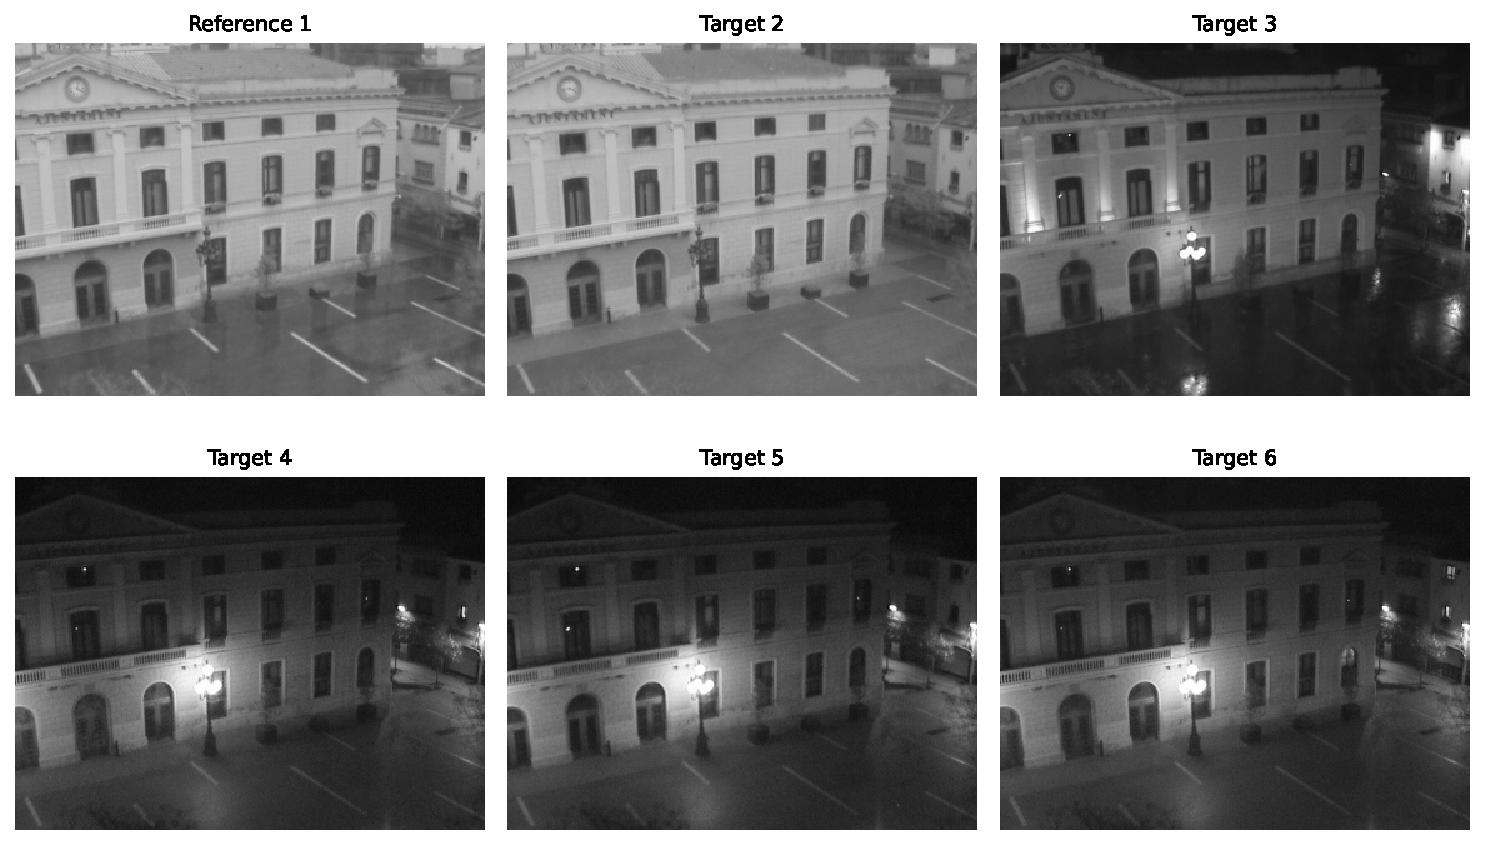
\includegraphics[width=\textwidth]{evidence/hp_00.pdf}
\caption{Actual reference and all evaluated targets for i\_ajuntament.}\label{fig:hp-scene-0}\end{figure}

\begin{table}[H]\centering\small
\caption{Saved oracle-pair support and corner error for i\_ajuntament.}\label{tab:hp-pairs-0}
\begin{tabular}{lrrrrrr}\toprule
Target & SIFT I & SIFT E & SIFT H5 & SP+LG I & SP+LG E & SP+LG H5 \\
\midrule
2 & 176 & 0.50 & yes & 366 & 0.71 & yes \\
3 & 9 & -- & no & 256 & 0.85 & yes \\
4 & 5 & -- & no & 193 & 0.93 & yes \\
5 & 12 & -- & no & 179 & 3.86 & yes \\
6 & 7 & -- & no & 193 & 2.33 & yes \\
\bottomrule\end{tabular}\end{table}


SIFT obtains 1 of five successful oracle homographies; SP+LG obtains 5 of five. The paired comparison contains 4 learned-only successes and 0 SIFT-only successes. Median inlier counts are 9.0 and 193.0, respectively. These support counts are computed from different tentative correspondence sets, so their magnitudes alone do not establish a more accurate mapping.

\begin{table}[H]\centering\small
\caption{Search and anchoring outcomes for the same five targets.}\label{tab:hp-end-0}
\begin{tabular}{lrrr}\toprule
Method & Rank-1 correct & Correctly verified & End-to-end H5 \\
\midrule
SIFT & 3/5 & 1/5 & 1/5 \\
SP+LG & 5/5 & 5/5 & 5/5 \\
Full & 5/5 & 5/5 & 5/5 \\
\bottomrule\end{tabular}\end{table}


The full hierarchy correctly verifies 5 of these five queries after searching the mixed 24-reference gallery. Its end-to-end column includes candidate selection and homography accuracy; the oracle table supplies the true reference directly. Any difference between those columns is therefore a search or decision effect rather than an additional illumination observation. The sequence remains one physical source of correlated targets, so five outcomes should not be treated as five independently sampled places.

\section{Sequence i\_autannes}

This sequence belongs to the illumination subset and contributes five reference-to-target pairs. Its identity is reserved for the projection-head training split; learned components in the main A--D comparison retain their original pretrained weights in either case.

\begin{figure}[H]\centering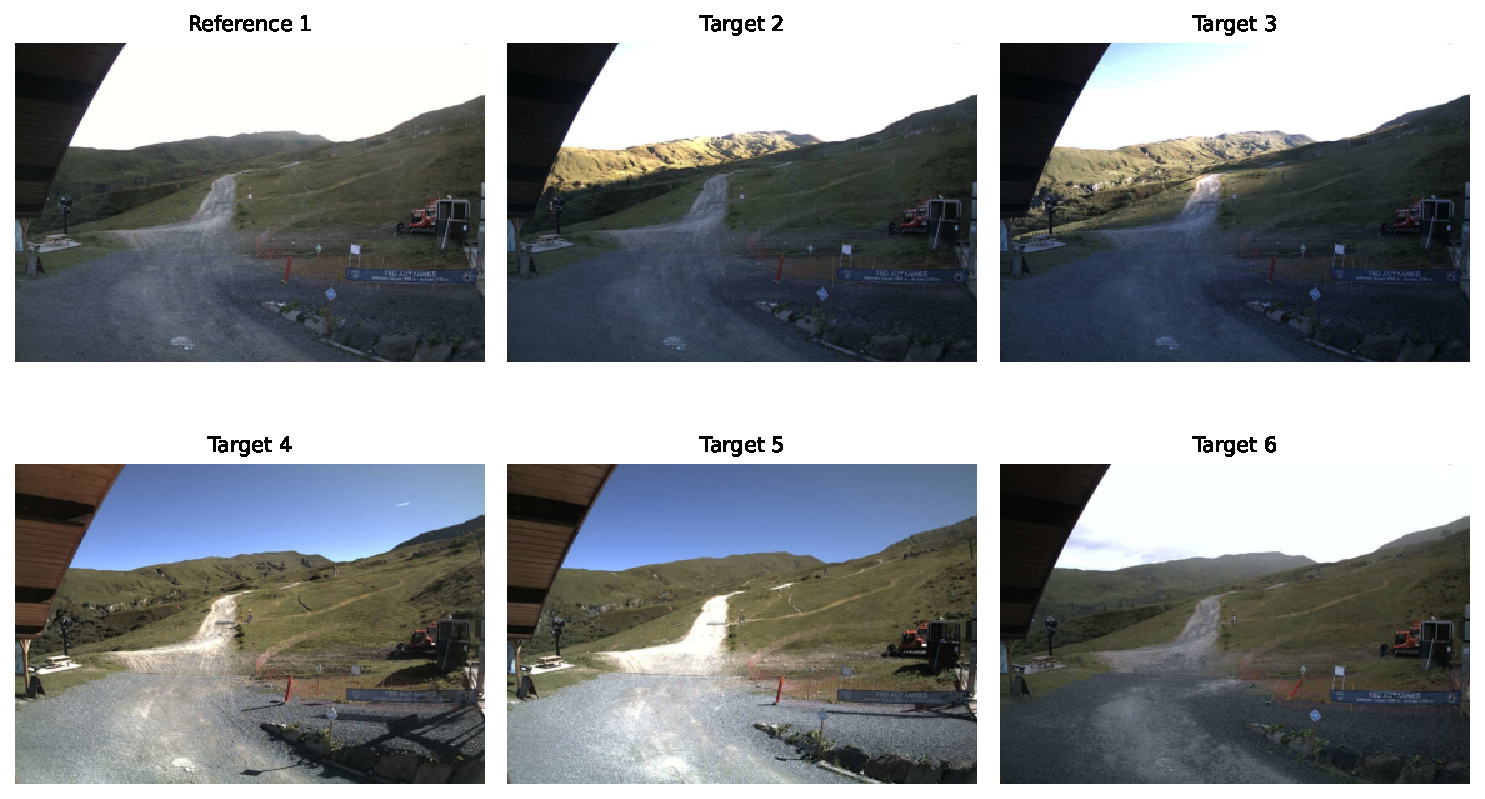
\includegraphics[width=\textwidth]{evidence/hp_01.pdf}
\caption{Actual reference and all evaluated targets for i\_autannes.}\label{fig:hp-scene-1}\end{figure}

\begin{table}[H]\centering\small
\caption{Saved oracle-pair support and corner error for i\_autannes.}\label{tab:hp-pairs-1}
\begin{tabular}{lrrrrrr}\toprule
Target & SIFT I & SIFT E & SIFT H5 & SP+LG I & SP+LG E & SP+LG H5 \\
\midrule
2 & 122 & 0.39 & yes & 335 & 0.54 & yes \\
3 & 60 & 6.79 & no & 305 & 0.83 & yes \\
4 & 19 & 1.25 & yes & 173 & 3.11 & yes \\
5 & 9 & 2.38 & no & 221 & 1.46 & yes \\
6 & 57 & 1.56 & yes & 315 & 0.61 & yes \\
\bottomrule\end{tabular}\end{table}


SIFT obtains 3 of five successful oracle homographies; SP+LG obtains 5 of five. The paired comparison contains 2 learned-only successes and 0 SIFT-only successes. Median inlier counts are 57.0 and 305.0, respectively. These support counts are computed from different tentative correspondence sets, so their magnitudes alone do not establish a more accurate mapping.

\begin{table}[H]\centering\small
\caption{Search and anchoring outcomes for the same five targets.}\label{tab:hp-end-1}
\begin{tabular}{lrrr}\toprule
Method & Rank-1 correct & Correctly verified & End-to-end H5 \\
\midrule
SIFT & 5/5 & 4/5 & 3/5 \\
SP+LG & 5/5 & 5/5 & 5/5 \\
Full & 5/5 & 5/5 & 5/5 \\
\bottomrule\end{tabular}\end{table}


The full hierarchy correctly verifies 5 of these five queries after searching the mixed 24-reference gallery. Its end-to-end column includes candidate selection and homography accuracy; the oracle table supplies the true reference directly. Any difference between those columns is therefore a search or decision effect rather than an additional illumination observation. The sequence remains one physical source of correlated targets, so five outcomes should not be treated as five independently sampled places.

\section{Sequence i\_bologna}

This sequence belongs to the illumination subset and contributes five reference-to-target pairs. Its identity is reserved for the projection-head training split; learned components in the main A--D comparison retain their original pretrained weights in either case.

\begin{figure}[H]\centering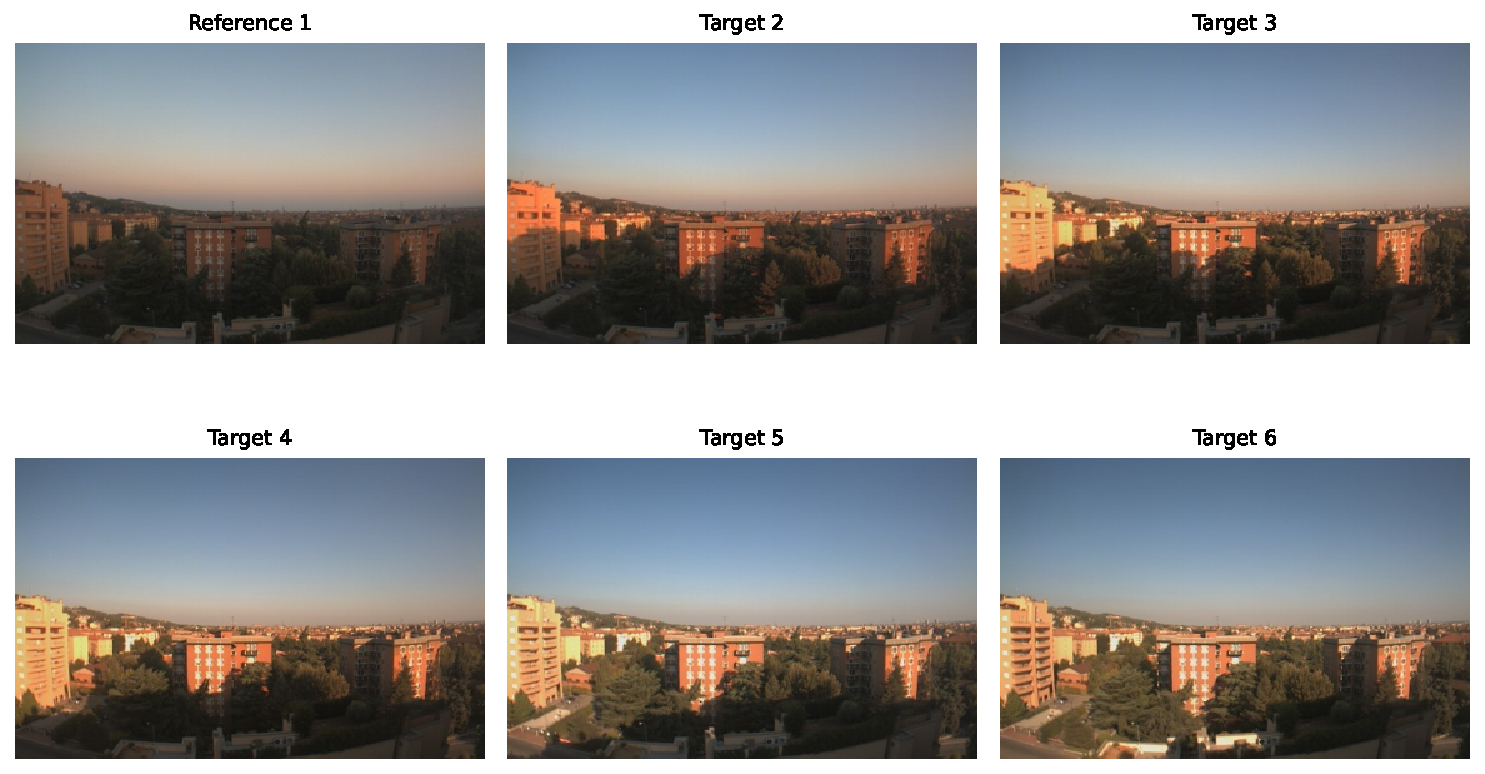
\includegraphics[width=\textwidth]{evidence/hp_02.pdf}
\caption{Actual reference and all evaluated targets for i\_bologna.}\label{fig:hp-scene-2}\end{figure}

\begin{table}[H]\centering\small
\caption{Saved oracle-pair support and corner error for i\_bologna.}\label{tab:hp-pairs-2}
\begin{tabular}{lrrrrrr}\toprule
Target & SIFT I & SIFT E & SIFT H5 & SP+LG I & SP+LG E & SP+LG H5 \\
\midrule
2 & 80 & 0.80 & yes & 366 & 0.64 & yes \\
3 & 43 & 1.85 & yes & 349 & 0.38 & yes \\
4 & 48 & 0.99 & yes & 336 & 0.65 & yes \\
5 & 48 & 2.28 & yes & 261 & 1.82 & yes \\
6 & 35 & 1.03 & yes & 308 & 1.31 & yes \\
\bottomrule\end{tabular}\end{table}


SIFT obtains 5 of five successful oracle homographies; SP+LG obtains 5 of five. The paired comparison contains 0 learned-only successes and 0 SIFT-only successes. Median inlier counts are 48.0 and 336.0, respectively. These support counts are computed from different tentative correspondence sets, so their magnitudes alone do not establish a more accurate mapping.

\begin{table}[H]\centering\small
\caption{Search and anchoring outcomes for the same five targets.}\label{tab:hp-end-2}
\begin{tabular}{lrrr}\toprule
Method & Rank-1 correct & Correctly verified & End-to-end H5 \\
\midrule
SIFT & 5/5 & 5/5 & 5/5 \\
SP+LG & 5/5 & 5/5 & 5/5 \\
Full & 5/5 & 5/5 & 5/5 \\
\bottomrule\end{tabular}\end{table}


The full hierarchy correctly verifies 5 of these five queries after searching the mixed 24-reference gallery. Its end-to-end column includes candidate selection and homography accuracy; the oracle table supplies the true reference directly. Any difference between those columns is therefore a search or decision effect rather than an additional illumination observation. The sequence remains one physical source of correlated targets, so five outcomes should not be treated as five independently sampled places.

\section{Sequence i\_books}

This sequence belongs to the illumination subset and contributes five reference-to-target pairs. Its identity is reserved for the projection-head training split; learned components in the main A--D comparison retain their original pretrained weights in either case.

\begin{figure}[H]\centering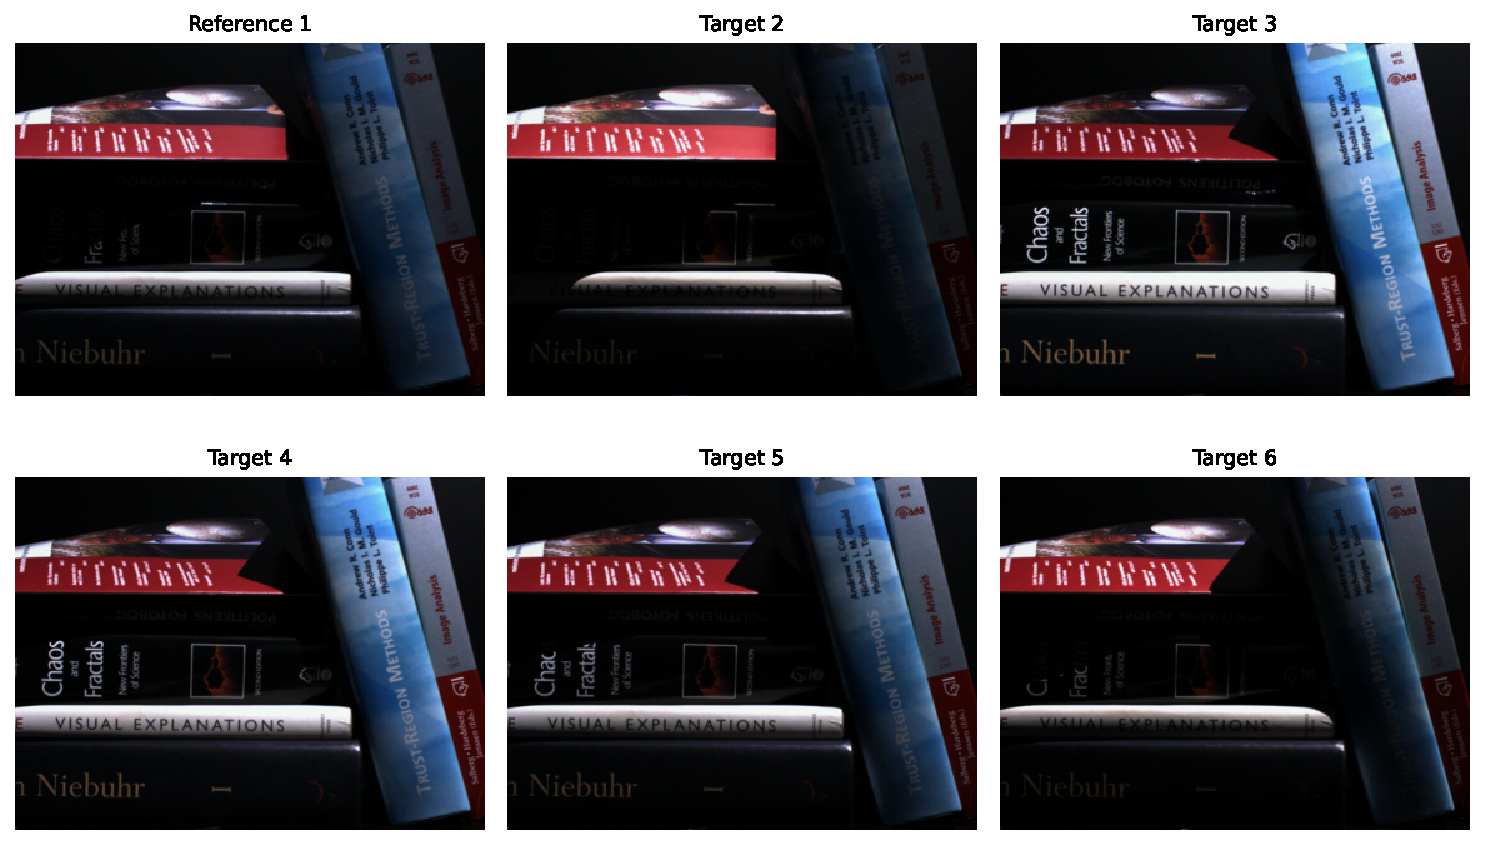
\includegraphics[width=\textwidth]{evidence/hp_03.pdf}
\caption{Actual reference and all evaluated targets for i\_books.}\label{fig:hp-scene-3}\end{figure}

\begin{table}[H]\centering\small
\caption{Saved oracle-pair support and corner error for i\_books.}\label{tab:hp-pairs-3}
\begin{tabular}{lrrrrrr}\toprule
Target & SIFT I & SIFT E & SIFT H5 & SP+LG I & SP+LG E & SP+LG H5 \\
\midrule
2 & 188 & 0.76 & yes & 421 & 0.20 & yes \\
3 & 164 & 0.68 & yes & 429 & 0.24 & yes \\
4 & 202 & 0.89 & yes & 438 & 0.31 & yes \\
5 & 234 & 0.09 & yes & 441 & 0.21 & yes \\
6 & 267 & 0.33 & yes & 431 & 0.27 & yes \\
\bottomrule\end{tabular}\end{table}


SIFT obtains 5 of five successful oracle homographies; SP+LG obtains 5 of five. The paired comparison contains 0 learned-only successes and 0 SIFT-only successes. Median inlier counts are 202.0 and 431.0, respectively. These support counts are computed from different tentative correspondence sets, so their magnitudes alone do not establish a more accurate mapping.

\begin{table}[H]\centering\small
\caption{Search and anchoring outcomes for the same five targets.}\label{tab:hp-end-3}
\begin{tabular}{lrrr}\toprule
Method & Rank-1 correct & Correctly verified & End-to-end H5 \\
\midrule
SIFT & 5/5 & 5/5 & 5/5 \\
SP+LG & 5/5 & 5/5 & 5/5 \\
Full & 5/5 & 5/5 & 5/5 \\
\bottomrule\end{tabular}\end{table}


The full hierarchy correctly verifies 5 of these five queries after searching the mixed 24-reference gallery. Its end-to-end column includes candidate selection and homography accuracy; the oracle table supplies the true reference directly. Any difference between those columns is therefore a search or decision effect rather than an additional illumination observation. The sequence remains one physical source of correlated targets, so five outcomes should not be treated as five independently sampled places.

\section{Sequence i\_boutique}

This sequence belongs to the illumination subset and contributes five reference-to-target pairs. Its identity is held out from projection-head training; learned components in the main A--D comparison retain their original pretrained weights in either case.

\begin{figure}[H]\centering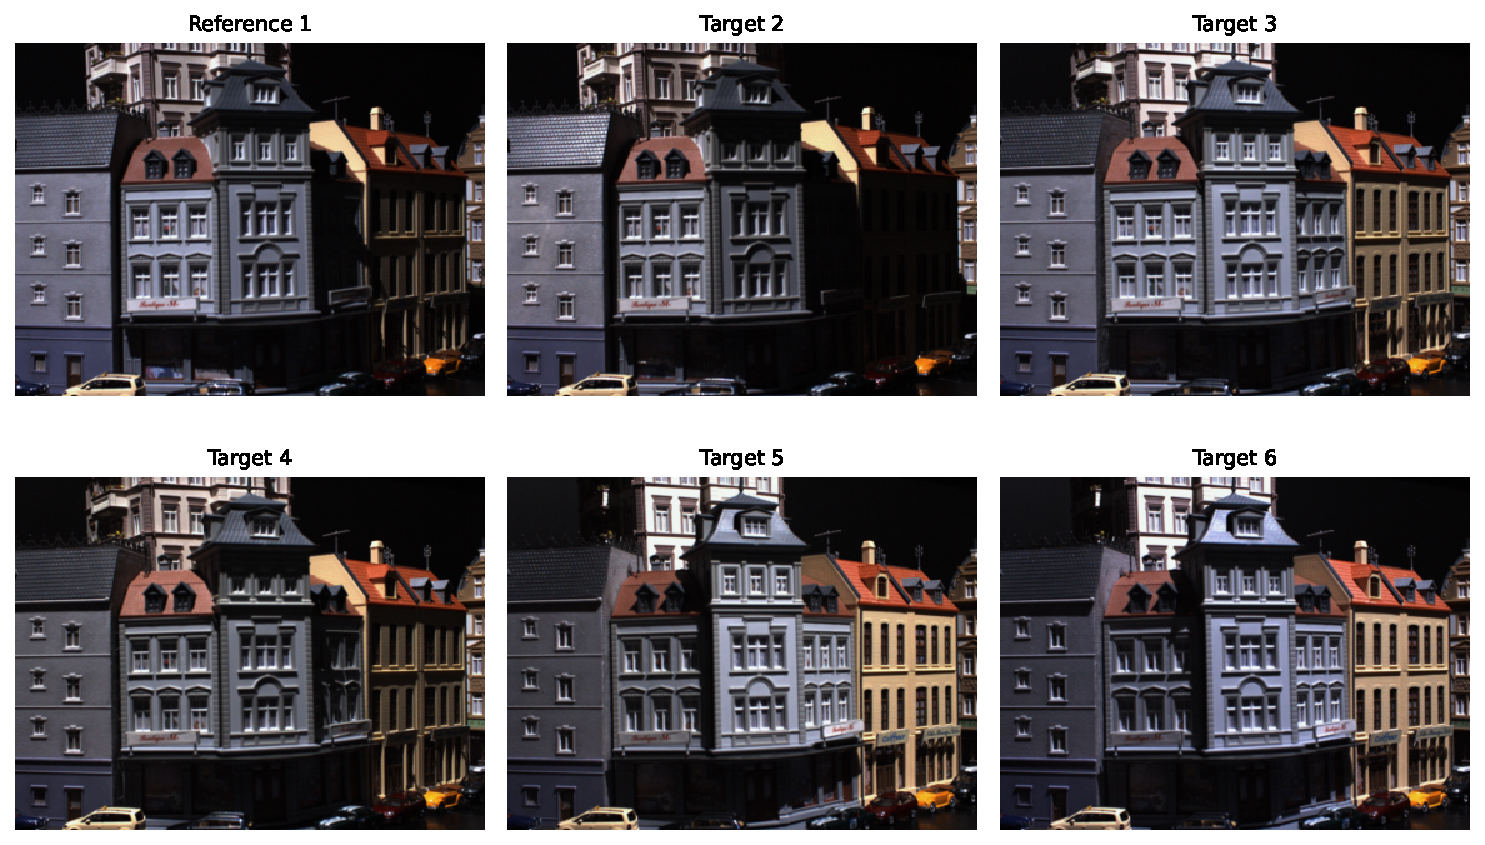
\includegraphics[width=\textwidth]{evidence/hp_04.pdf}
\caption{Actual reference and all evaluated targets for i\_boutique.}\label{fig:hp-scene-4}\end{figure}

\begin{table}[H]\centering\small
\caption{Saved oracle-pair support and corner error for i\_boutique.}\label{tab:hp-pairs-4}
\begin{tabular}{lrrrrrr}\toprule
Target & SIFT I & SIFT E & SIFT H5 & SP+LG I & SP+LG E & SP+LG H5 \\
\midrule
2 & 157 & 0.27 & yes & 371 & 0.32 & yes \\
3 & 51 & 0.29 & yes & 272 & 0.45 & yes \\
4 & 70 & 0.68 & yes & 317 & 0.51 & yes \\
5 & 7 & -- & no & 248 & 0.66 & yes \\
6 & 8 & 0.57 & no & 226 & 0.80 & yes \\
\bottomrule\end{tabular}\end{table}


SIFT obtains 3 of five successful oracle homographies; SP+LG obtains 5 of five. The paired comparison contains 2 learned-only successes and 0 SIFT-only successes. Median inlier counts are 51.0 and 272.0, respectively. These support counts are computed from different tentative correspondence sets, so their magnitudes alone do not establish a more accurate mapping.

\begin{table}[H]\centering\small
\caption{Search and anchoring outcomes for the same five targets.}\label{tab:hp-end-4}
\begin{tabular}{lrrr}\toprule
Method & Rank-1 correct & Correctly verified & End-to-end H5 \\
\midrule
SIFT & 4/5 & 3/5 & 3/5 \\
SP+LG & 5/5 & 5/5 & 5/5 \\
Full & 5/5 & 5/5 & 5/5 \\
\bottomrule\end{tabular}\end{table}


The full hierarchy correctly verifies 5 of these five queries after searching the mixed 24-reference gallery. Its end-to-end column includes candidate selection and homography accuracy; the oracle table supplies the true reference directly. Any difference between those columns is therefore a search or decision effect rather than an additional illumination observation. The sequence remains one physical source of correlated targets, so five outcomes should not be treated as five independently sampled places.

\section{Sequence i\_bridger}

This sequence belongs to the illumination subset and contributes five reference-to-target pairs. Its identity is held out from projection-head training; learned components in the main A--D comparison retain their original pretrained weights in either case.

\begin{figure}[H]\centering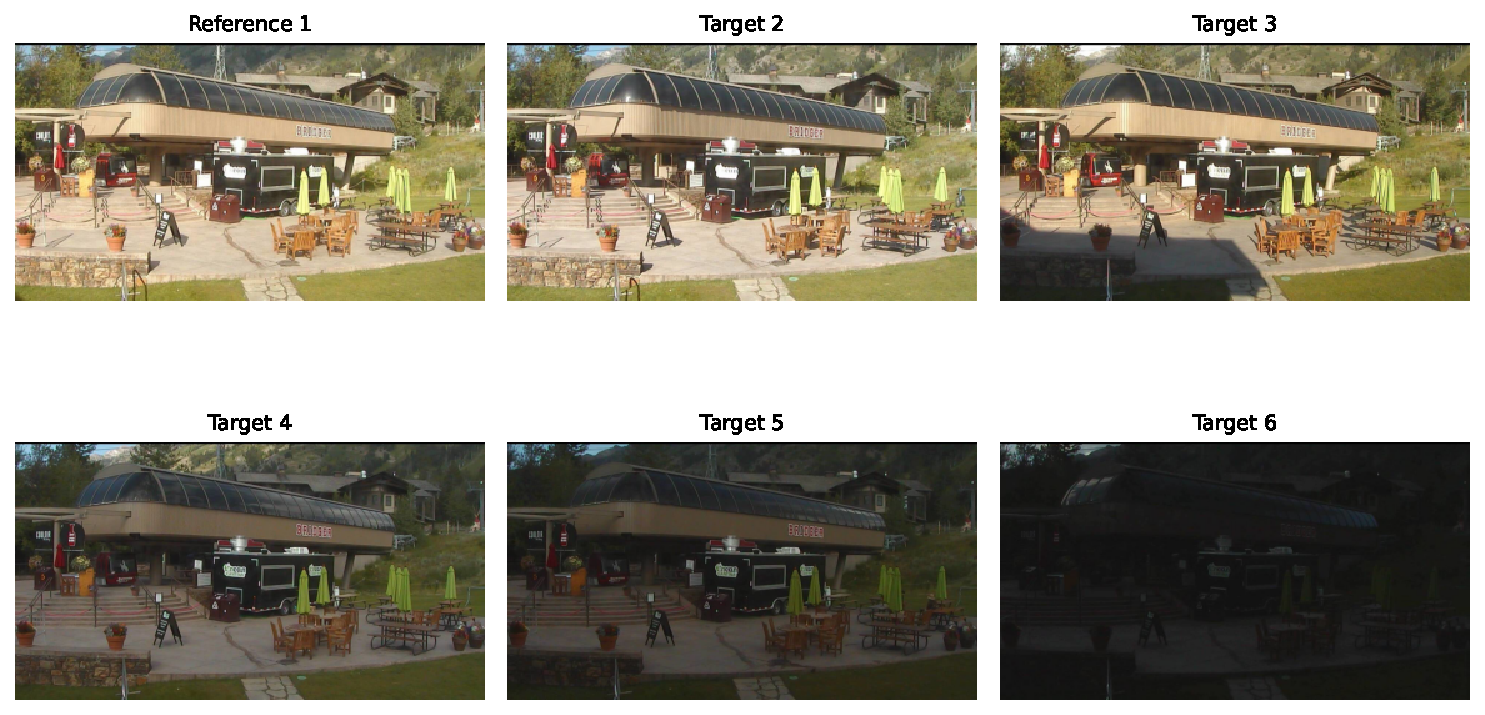
\includegraphics[width=\textwidth]{evidence/hp_05.pdf}
\caption{Actual reference and all evaluated targets for i\_bridger.}\label{fig:hp-scene-5}\end{figure}

\begin{table}[H]\centering\small
\caption{Saved oracle-pair support and corner error for i\_bridger.}\label{tab:hp-pairs-5}
\begin{tabular}{lrrrrrr}\toprule
Target & SIFT I & SIFT E & SIFT H5 & SP+LG I & SP+LG E & SP+LG H5 \\
\midrule
2 & 127 & 0.43 & yes & 339 & 0.29 & yes \\
3 & 99 & 0.42 & yes & 318 & 0.45 & yes \\
4 & 89 & 0.23 & yes & 341 & 0.39 & yes \\
5 & 56 & 1.25 & yes & 308 & 0.61 & yes \\
6 & 4 & -- & no & 172 & 1.27 & yes \\
\bottomrule\end{tabular}\end{table}


SIFT obtains 4 of five successful oracle homographies; SP+LG obtains 5 of five. The paired comparison contains 1 learned-only success and 0 SIFT-only successes. Median inlier counts are 89.0 and 318.0, respectively. These support counts are computed from different tentative correspondence sets, so their magnitudes alone do not establish a more accurate mapping.

\begin{table}[H]\centering\small
\caption{Search and anchoring outcomes for the same five targets.}\label{tab:hp-end-5}
\begin{tabular}{lrrr}\toprule
Method & Rank-1 correct & Correctly verified & End-to-end H5 \\
\midrule
SIFT & 4/5 & 4/5 & 4/5 \\
SP+LG & 5/5 & 5/5 & 5/5 \\
Full & 5/5 & 5/5 & 5/5 \\
\bottomrule\end{tabular}\end{table}


The full hierarchy correctly verifies 5 of these five queries after searching the mixed 24-reference gallery. Its end-to-end column includes candidate selection and homography accuracy; the oracle table supplies the true reference directly. Any difference between those columns is therefore a search or decision effect rather than an additional illumination observation. The sequence remains one physical source of correlated targets, so five outcomes should not be treated as five independently sampled places.

\section{Sequence i\_brooklyn}

This sequence belongs to the illumination subset and contributes five reference-to-target pairs. Its identity is held out from projection-head training; learned components in the main A--D comparison retain their original pretrained weights in either case.

\begin{figure}[H]\centering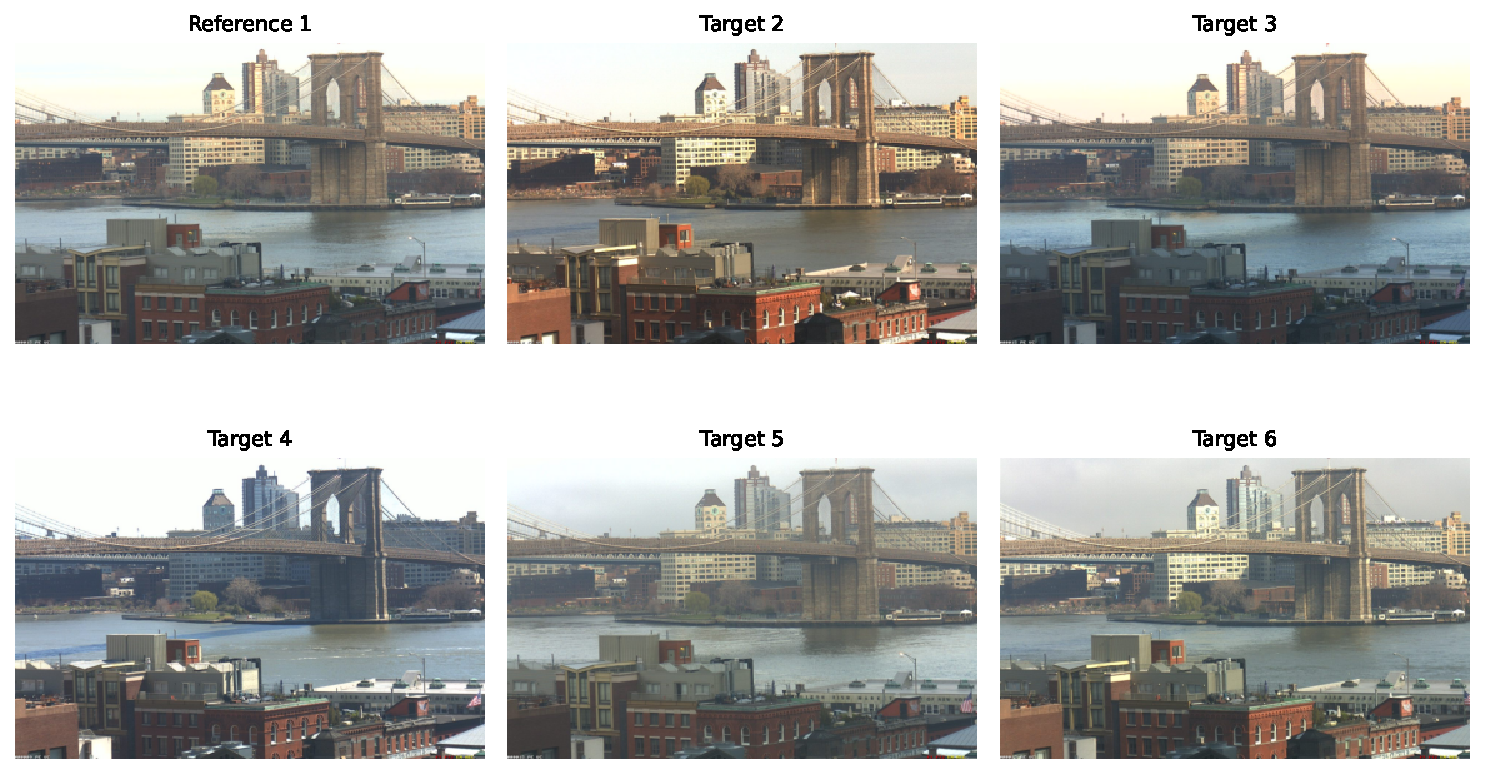
\includegraphics[width=\textwidth]{evidence/hp_06.pdf}
\caption{Actual reference and all evaluated targets for i\_brooklyn.}\label{fig:hp-scene-6}\end{figure}

\begin{table}[H]\centering\small
\caption{Saved oracle-pair support and corner error for i\_brooklyn.}\label{tab:hp-pairs-6}
\begin{tabular}{lrrrrrr}\toprule
Target & SIFT I & SIFT E & SIFT H5 & SP+LG I & SP+LG E & SP+LG H5 \\
\midrule
2 & 140 & 0.71 & yes & 296 & 0.48 & yes \\
3 & 232 & 1.73 & yes & 396 & 1.62 & yes \\
4 & 15 & 2.53 & yes & 295 & 1.03 & yes \\
5 & 244 & 2.00 & yes & 411 & 1.96 & yes \\
6 & 121 & 2.45 & yes & 322 & 1.85 & yes \\
\bottomrule\end{tabular}\end{table}


SIFT obtains 5 of five successful oracle homographies; SP+LG obtains 5 of five. The paired comparison contains 0 learned-only successes and 0 SIFT-only successes. Median inlier counts are 140.0 and 322.0, respectively. These support counts are computed from different tentative correspondence sets, so their magnitudes alone do not establish a more accurate mapping.

\begin{table}[H]\centering\small
\caption{Search and anchoring outcomes for the same five targets.}\label{tab:hp-end-6}
\begin{tabular}{lrrr}\toprule
Method & Rank-1 correct & Correctly verified & End-to-end H5 \\
\midrule
SIFT & 5/5 & 5/5 & 5/5 \\
SP+LG & 5/5 & 5/5 & 5/5 \\
Full & 5/5 & 5/5 & 5/5 \\
\bottomrule\end{tabular}\end{table}


The full hierarchy correctly verifies 5 of these five queries after searching the mixed 24-reference gallery. Its end-to-end column includes candidate selection and homography accuracy; the oracle table supplies the true reference directly. Any difference between those columns is therefore a search or decision effect rather than an additional illumination observation. The sequence remains one physical source of correlated targets, so five outcomes should not be treated as five independently sampled places.

\section{Sequence i\_castle}

This sequence belongs to the illumination subset and contributes five reference-to-target pairs. Its identity is held out from projection-head training; learned components in the main A--D comparison retain their original pretrained weights in either case.

\begin{figure}[H]\centering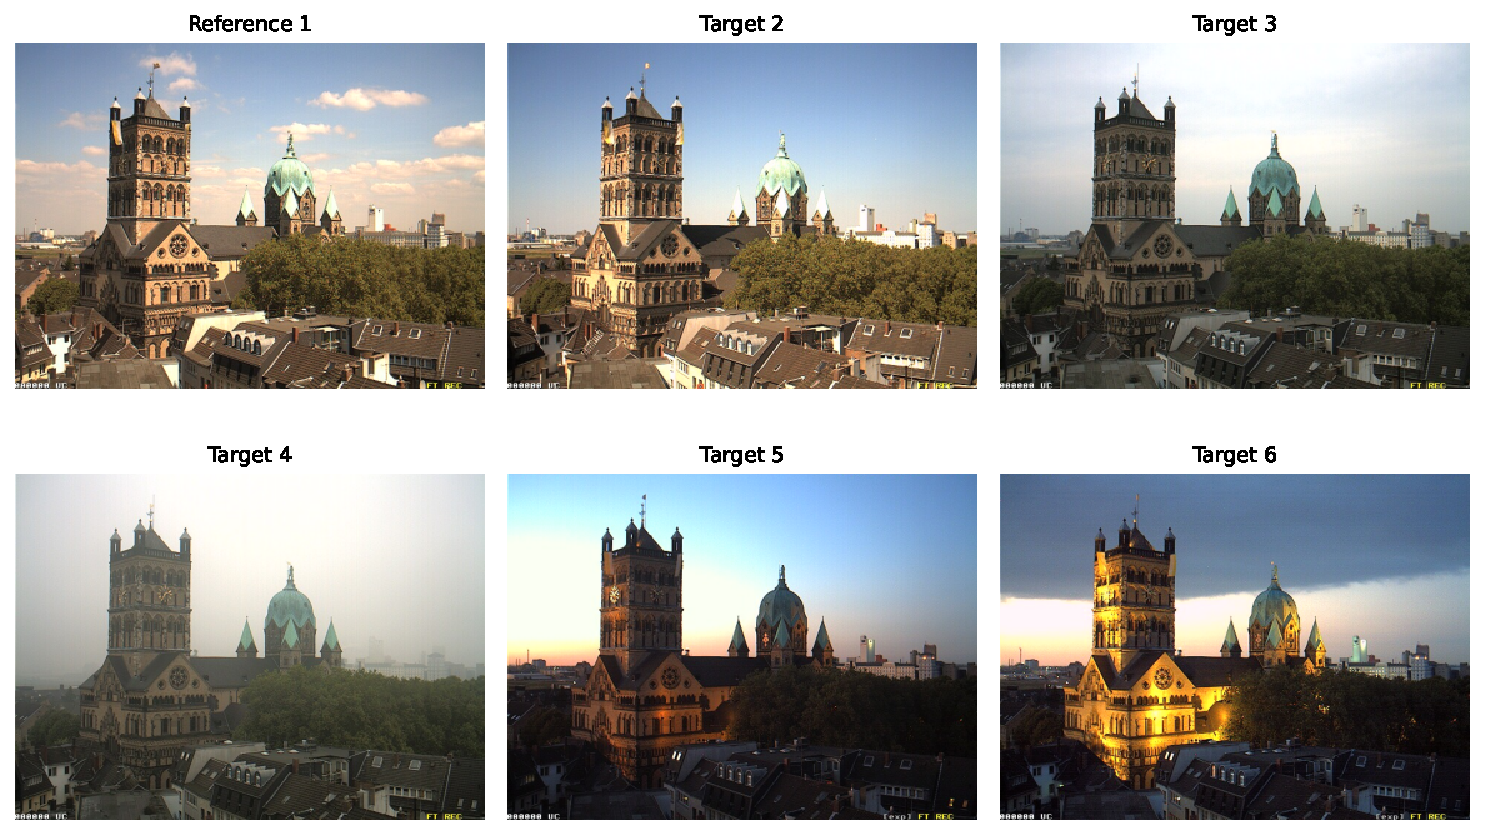
\includegraphics[width=\textwidth]{evidence/hp_07.pdf}
\caption{Actual reference and all evaluated targets for i\_castle.}\label{fig:hp-scene-7}\end{figure}

\begin{table}[H]\centering\small
\caption{Saved oracle-pair support and corner error for i\_castle.}\label{tab:hp-pairs-7}
\begin{tabular}{lrrrrrr}\toprule
Target & SIFT I & SIFT E & SIFT H5 & SP+LG I & SP+LG E & SP+LG H5 \\
\midrule
2 & 12 & 3.85 & yes & 282 & 1.30 & yes \\
3 & 49 & 0.96 & yes & 359 & 0.83 & yes \\
4 & 53 & 1.19 & yes & 299 & 1.14 & yes \\
5 & 10 & 5.27 & no & 295 & 0.64 & yes \\
6 & 12 & 1.02 & yes & 290 & 0.48 & yes \\
\bottomrule\end{tabular}\end{table}


SIFT obtains 4 of five successful oracle homographies; SP+LG obtains 5 of five. The paired comparison contains 1 learned-only success and 0 SIFT-only successes. Median inlier counts are 12.0 and 295.0, respectively. These support counts are computed from different tentative correspondence sets, so their magnitudes alone do not establish a more accurate mapping.

\begin{table}[H]\centering\small
\caption{Search and anchoring outcomes for the same five targets.}\label{tab:hp-end-7}
\begin{tabular}{lrrr}\toprule
Method & Rank-1 correct & Correctly verified & End-to-end H5 \\
\midrule
SIFT & 5/5 & 4/5 & 4/5 \\
SP+LG & 5/5 & 5/5 & 5/5 \\
Full & 5/5 & 5/5 & 5/5 \\
\bottomrule\end{tabular}\end{table}


The full hierarchy correctly verifies 5 of these five queries after searching the mixed 24-reference gallery. Its end-to-end column includes candidate selection and homography accuracy; the oracle table supplies the true reference directly. Any difference between those columns is therefore a search or decision effect rather than an additional illumination observation. The sequence remains one physical source of correlated targets, so five outcomes should not be treated as five independently sampled places.

\section{Sequence i\_chestnuts}

This sequence belongs to the illumination subset and contributes five reference-to-target pairs. Its identity is held out from projection-head training; learned components in the main A--D comparison retain their original pretrained weights in either case.

\begin{figure}[H]\centering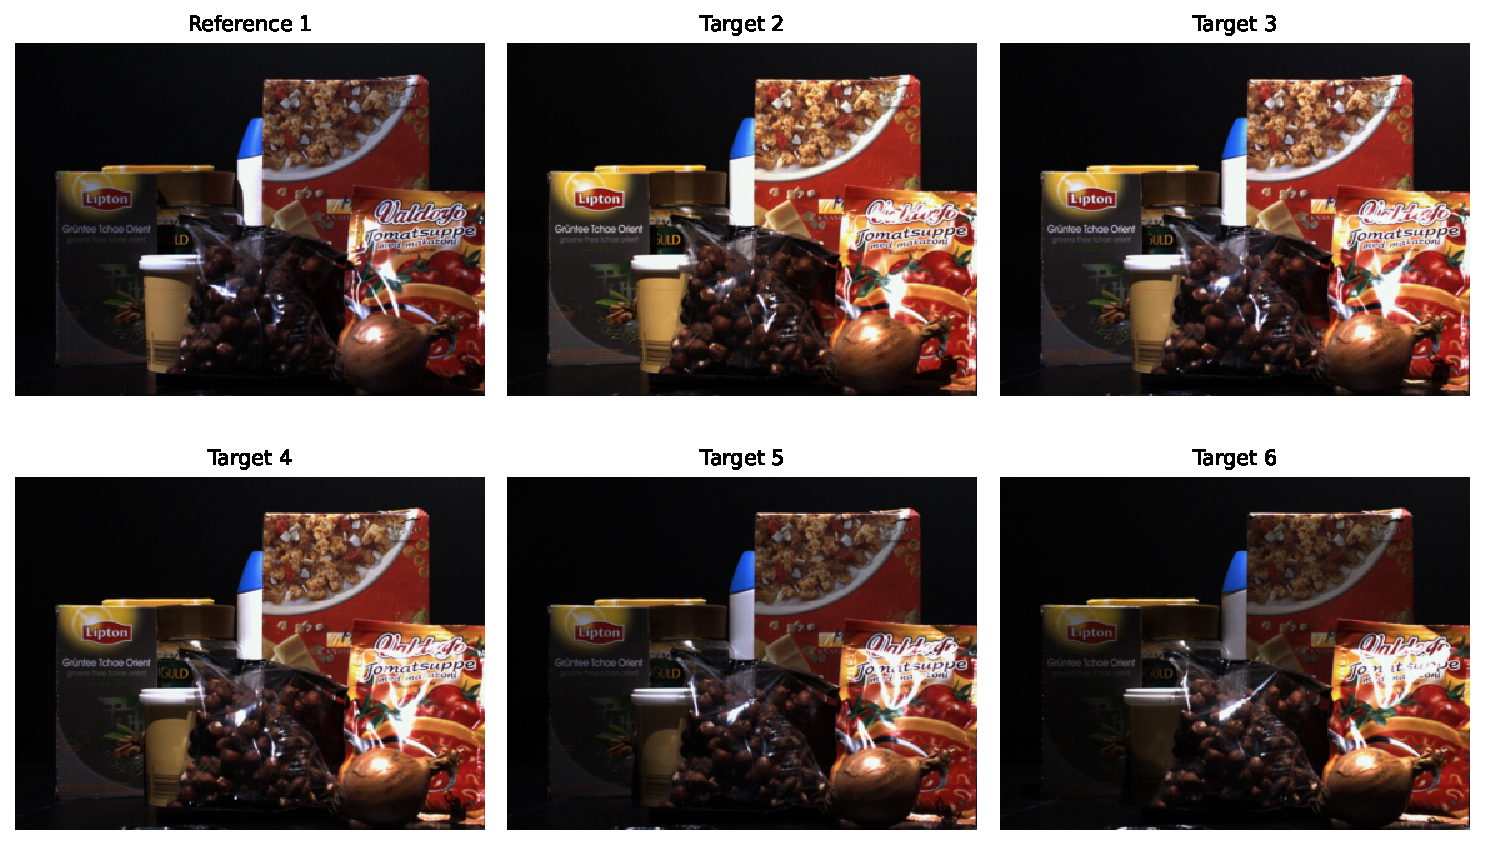
\includegraphics[width=\textwidth]{evidence/hp_08.pdf}
\caption{Actual reference and all evaluated targets for i\_chestnuts.}\label{fig:hp-scene-8}\end{figure}

\begin{table}[H]\centering\small
\caption{Saved oracle-pair support and corner error for i\_chestnuts.}\label{tab:hp-pairs-8}
\begin{tabular}{lrrrrrr}\toprule
Target & SIFT I & SIFT E & SIFT H5 & SP+LG I & SP+LG E & SP+LG H5 \\
\midrule
2 & 153 & 0.25 & yes & 317 & 0.73 & yes \\
3 & 150 & 0.36 & yes & 370 & 0.23 & yes \\
4 & 155 & 0.25 & yes & 342 & 0.28 & yes \\
5 & 121 & 0.42 & yes & 317 & 0.31 & yes \\
6 & 56 & 0.63 & yes & 273 & 0.49 & yes \\
\bottomrule\end{tabular}\end{table}


SIFT obtains 5 of five successful oracle homographies; SP+LG obtains 5 of five. The paired comparison contains 0 learned-only successes and 0 SIFT-only successes. Median inlier counts are 150.0 and 317.0, respectively. These support counts are computed from different tentative correspondence sets, so their magnitudes alone do not establish a more accurate mapping.

\begin{table}[H]\centering\small
\caption{Search and anchoring outcomes for the same five targets.}\label{tab:hp-end-8}
\begin{tabular}{lrrr}\toprule
Method & Rank-1 correct & Correctly verified & End-to-end H5 \\
\midrule
SIFT & 5/5 & 5/5 & 5/5 \\
SP+LG & 5/5 & 5/5 & 5/5 \\
Full & 5/5 & 5/5 & 5/5 \\
\bottomrule\end{tabular}\end{table}


The full hierarchy correctly verifies 5 of these five queries after searching the mixed 24-reference gallery. Its end-to-end column includes candidate selection and homography accuracy; the oracle table supplies the true reference directly. Any difference between those columns is therefore a search or decision effect rather than an additional illumination observation. The sequence remains one physical source of correlated targets, so five outcomes should not be treated as five independently sampled places.

\section{Sequence i\_contruction}

This sequence belongs to the illumination subset and contributes five reference-to-target pairs. Its identity is held out from projection-head training; learned components in the main A--D comparison retain their original pretrained weights in either case.

\begin{figure}[H]\centering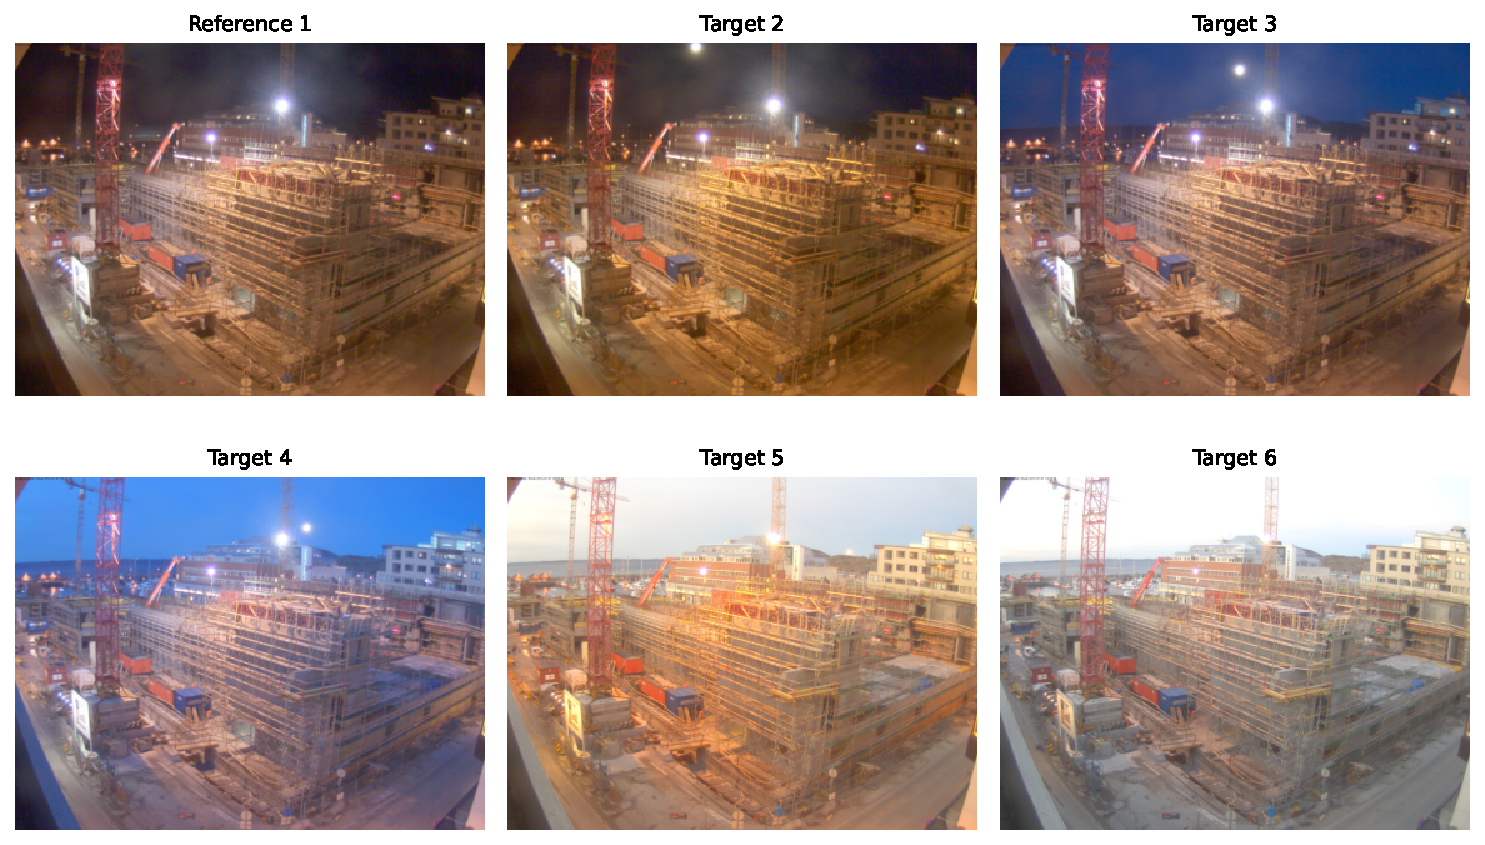
\includegraphics[width=\textwidth]{evidence/hp_09.pdf}
\caption{Actual reference and all evaluated targets for i\_contruction.}\label{fig:hp-scene-9}\end{figure}

\begin{table}[H]\centering\small
\caption{Saved oracle-pair support and corner error for i\_contruction.}\label{tab:hp-pairs-9}
\begin{tabular}{lrrrrrr}\toprule
Target & SIFT I & SIFT E & SIFT H5 & SP+LG I & SP+LG E & SP+LG H5 \\
\midrule
2 & 424 & 0.05 & yes & 462 & 0.07 & yes \\
3 & 414 & 0.05 & yes & 449 & 0.28 & yes \\
4 & 276 & 0.32 & yes & 392 & 0.15 & yes \\
5 & 70 & 0.46 & yes & 253 & 0.46 & yes \\
6 & 29 & 1.11 & yes & 236 & 0.54 & yes \\
\bottomrule\end{tabular}\end{table}


SIFT obtains 5 of five successful oracle homographies; SP+LG obtains 5 of five. The paired comparison contains 0 learned-only successes and 0 SIFT-only successes. Median inlier counts are 276.0 and 392.0, respectively. These support counts are computed from different tentative correspondence sets, so their magnitudes alone do not establish a more accurate mapping.

\begin{table}[H]\centering\small
\caption{Search and anchoring outcomes for the same five targets.}\label{tab:hp-end-9}
\begin{tabular}{lrrr}\toprule
Method & Rank-1 correct & Correctly verified & End-to-end H5 \\
\midrule
SIFT & 5/5 & 5/5 & 5/5 \\
SP+LG & 5/5 & 5/5 & 5/5 \\
Full & 5/5 & 5/5 & 5/5 \\
\bottomrule\end{tabular}\end{table}


The full hierarchy correctly verifies 5 of these five queries after searching the mixed 24-reference gallery. Its end-to-end column includes candidate selection and homography accuracy; the oracle table supplies the true reference directly. Any difference between those columns is therefore a search or decision effect rather than an additional illumination observation. The sequence remains one physical source of correlated targets, so five outcomes should not be treated as five independently sampled places.

\section{Sequence i\_crownday}

This sequence belongs to the illumination subset and contributes five reference-to-target pairs. Its identity is held out from projection-head training; learned components in the main A--D comparison retain their original pretrained weights in either case.

\begin{figure}[H]\centering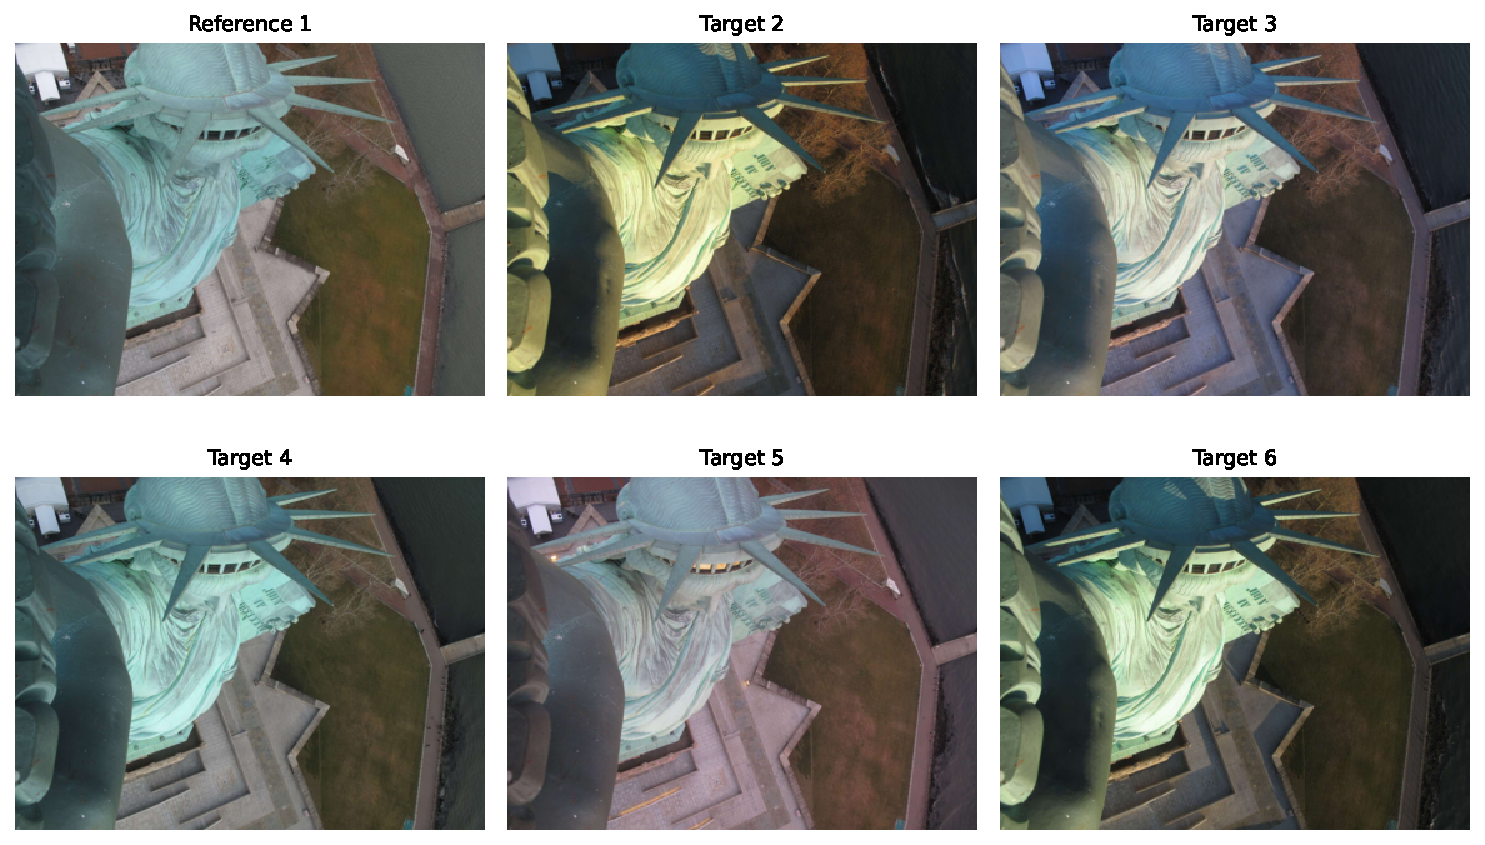
\includegraphics[width=\textwidth]{evidence/hp_10.pdf}
\caption{Actual reference and all evaluated targets for i\_crownday.}\label{fig:hp-scene-10}\end{figure}

\begin{table}[H]\centering\small
\caption{Saved oracle-pair support and corner error for i\_crownday.}\label{tab:hp-pairs-10}
\begin{tabular}{lrrrrrr}\toprule
Target & SIFT I & SIFT E & SIFT H5 & SP+LG I & SP+LG E & SP+LG H5 \\
\midrule
2 & 20 & 1.29 & yes & 272 & 0.48 & yes \\
3 & 37 & 2.11 & yes & 325 & 0.63 & yes \\
4 & 82 & 0.60 & yes & 350 & 0.37 & yes \\
5 & 181 & 0.68 & yes & 373 & 0.76 & yes \\
6 & 22 & 1.60 & yes & 274 & 0.29 & yes \\
\bottomrule\end{tabular}\end{table}


SIFT obtains 5 of five successful oracle homographies; SP+LG obtains 5 of five. The paired comparison contains 0 learned-only successes and 0 SIFT-only successes. Median inlier counts are 37.0 and 325.0, respectively. These support counts are computed from different tentative correspondence sets, so their magnitudes alone do not establish a more accurate mapping.

\begin{table}[H]\centering\small
\caption{Search and anchoring outcomes for the same five targets.}\label{tab:hp-end-10}
\begin{tabular}{lrrr}\toprule
Method & Rank-1 correct & Correctly verified & End-to-end H5 \\
\midrule
SIFT & 5/5 & 5/5 & 5/5 \\
SP+LG & 5/5 & 5/5 & 5/5 \\
Full & 5/5 & 5/5 & 5/5 \\
\bottomrule\end{tabular}\end{table}


The full hierarchy correctly verifies 5 of these five queries after searching the mixed 24-reference gallery. Its end-to-end column includes candidate selection and homography accuracy; the oracle table supplies the true reference directly. Any difference between those columns is therefore a search or decision effect rather than an additional illumination observation. The sequence remains one physical source of correlated targets, so five outcomes should not be treated as five independently sampled places.

\section{Sequence i\_crownnight}

This sequence belongs to the illumination subset and contributes five reference-to-target pairs. Its identity is held out from projection-head training; learned components in the main A--D comparison retain their original pretrained weights in either case.

\begin{figure}[H]\centering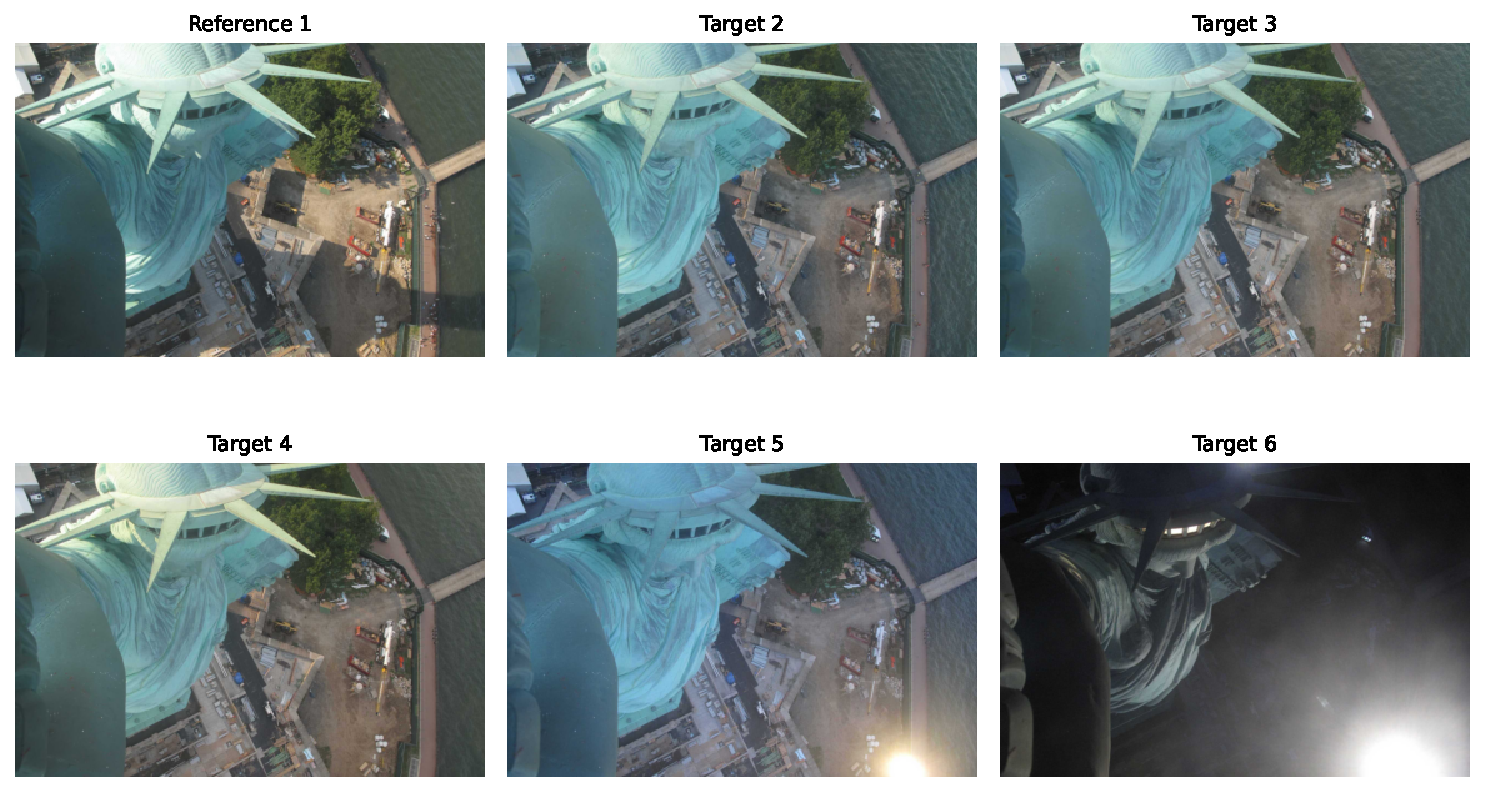
\includegraphics[width=\textwidth]{evidence/hp_11.pdf}
\caption{Actual reference and all evaluated targets for i\_crownnight.}\label{fig:hp-scene-11}\end{figure}

\begin{table}[H]\centering\small
\caption{Saved oracle-pair support and corner error for i\_crownnight.}\label{tab:hp-pairs-11}
\begin{tabular}{lrrrrrr}\toprule
Target & SIFT I & SIFT E & SIFT H5 & SP+LG I & SP+LG E & SP+LG H5 \\
\midrule
2 & 79 & 0.28 & yes & 343 & 0.47 & yes \\
3 & 65 & 0.78 & yes & 308 & 0.77 & yes \\
4 & 54 & 1.45 & yes & 327 & 0.20 & yes \\
5 & 34 & 0.33 & yes & 318 & 0.37 & yes \\
6 & 0 & -- & no & 119 & 1.95 & yes \\
\bottomrule\end{tabular}\end{table}


SIFT obtains 4 of five successful oracle homographies; SP+LG obtains 5 of five. The paired comparison contains 1 learned-only success and 0 SIFT-only successes. Median inlier counts are 54.0 and 318.0, respectively. These support counts are computed from different tentative correspondence sets, so their magnitudes alone do not establish a more accurate mapping.

\begin{table}[H]\centering\small
\caption{Search and anchoring outcomes for the same five targets.}\label{tab:hp-end-11}
\begin{tabular}{lrrr}\toprule
Method & Rank-1 correct & Correctly verified & End-to-end H5 \\
\midrule
SIFT & 3/5 & 3/5 & 3/5 \\
SP+LG & 4/5 & 4/5 & 4/5 \\
Full & 4/5 & 4/5 & 4/5 \\
\bottomrule\end{tabular}\end{table}


The full hierarchy correctly verifies 4 of these five queries after searching the mixed 24-reference gallery. Its end-to-end column includes candidate selection and homography accuracy; the oracle table supplies the true reference directly. Any difference between those columns is therefore a search or decision effect rather than an additional illumination observation. The sequence remains one physical source of correlated targets, so five outcomes should not be treated as five independently sampled places.

\section{Sequence v\_abstract}

This sequence belongs to the viewpoint subset and contributes five reference-to-target pairs. Its identity is reserved for the projection-head training split; learned components in the main A--D comparison retain their original pretrained weights in either case.

\begin{figure}[H]\centering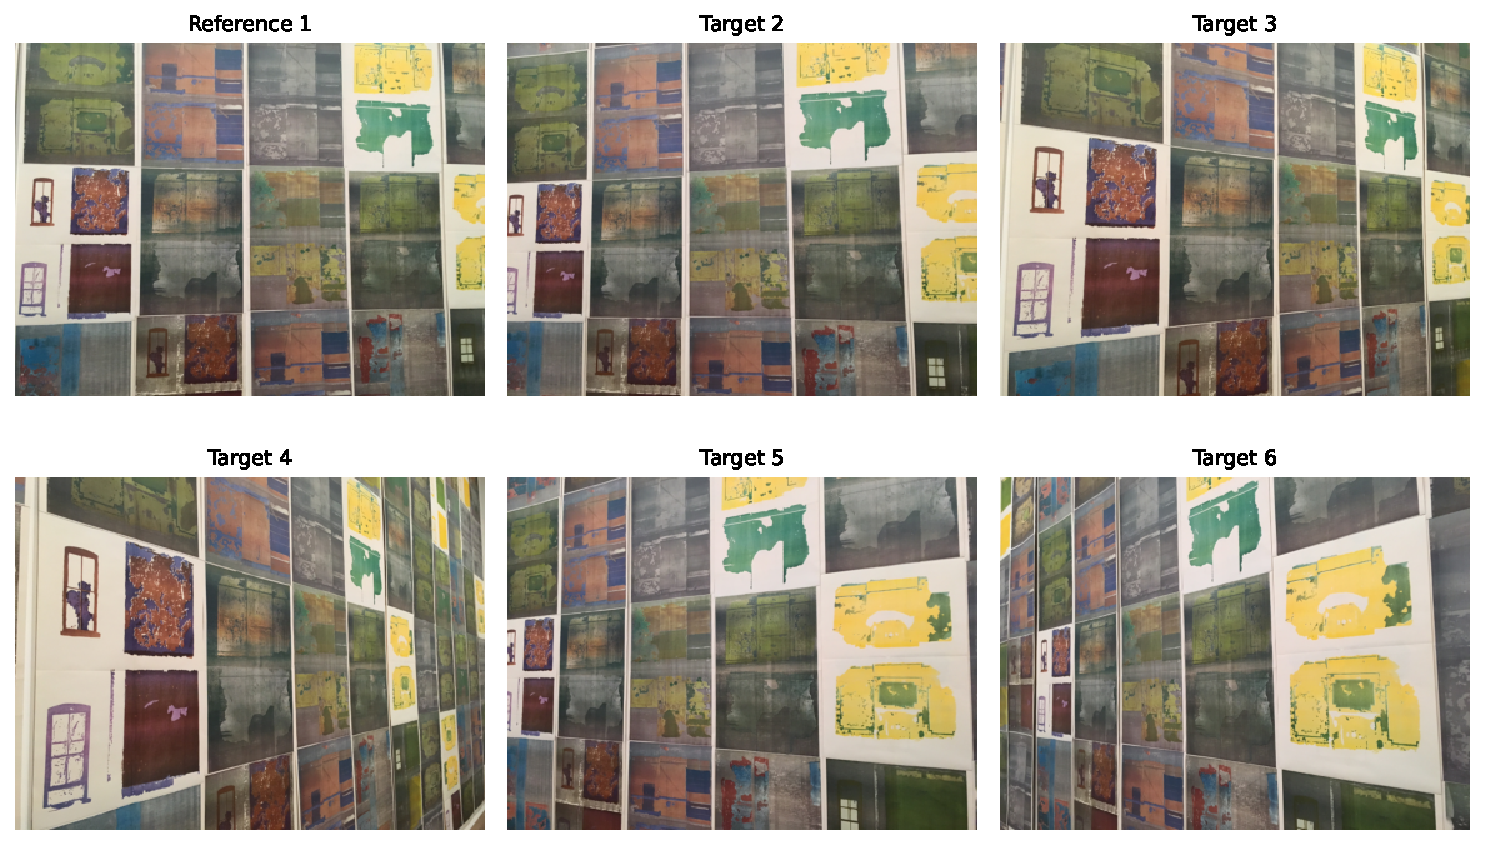
\includegraphics[width=\textwidth]{evidence/hp_12.pdf}
\caption{Actual reference and all evaluated targets for v\_abstract.}\label{fig:hp-scene-12}\end{figure}

\begin{table}[H]\centering\small
\caption{Saved oracle-pair support and corner error for v\_abstract.}\label{tab:hp-pairs-12}
\begin{tabular}{lrrrrrr}\toprule
Target & SIFT I & SIFT E & SIFT H5 & SP+LG I & SP+LG E & SP+LG H5 \\
\midrule
2 & 226 & 0.38 & yes & 373 & 0.20 & yes \\
3 & 181 & 0.61 & yes & 353 & 0.37 & yes \\
4 & 86 & 2.60 & yes & 215 & 1.96 & yes \\
5 & 130 & 1.50 & yes & 279 & 0.67 & yes \\
6 & 49 & 3.80 & yes & 189 & 1.80 & yes \\
\bottomrule\end{tabular}\end{table}


SIFT obtains 5 of five successful oracle homographies; SP+LG obtains 5 of five. The paired comparison contains 0 learned-only successes and 0 SIFT-only successes. Median inlier counts are 130.0 and 279.0, respectively. These support counts are computed from different tentative correspondence sets, so their magnitudes alone do not establish a more accurate mapping.

\begin{table}[H]\centering\small
\caption{Search and anchoring outcomes for the same five targets.}\label{tab:hp-end-12}
\begin{tabular}{lrrr}\toprule
Method & Rank-1 correct & Correctly verified & End-to-end H5 \\
\midrule
SIFT & 5/5 & 5/5 & 5/5 \\
SP+LG & 5/5 & 5/5 & 5/5 \\
Full & 5/5 & 5/5 & 5/5 \\
\bottomrule\end{tabular}\end{table}


The full hierarchy correctly verifies 5 of these five queries after searching the mixed 24-reference gallery. Its end-to-end column includes candidate selection and homography accuracy; the oracle table supplies the true reference directly. Any difference between those columns is therefore a search or decision effect rather than an additional illumination observation. The sequence remains one physical source of correlated targets, so five outcomes should not be treated as five independently sampled places.

\section{Sequence v\_adam}

This sequence belongs to the viewpoint subset and contributes five reference-to-target pairs. Its identity is reserved for the projection-head training split; learned components in the main A--D comparison retain their original pretrained weights in either case.

\begin{figure}[H]\centering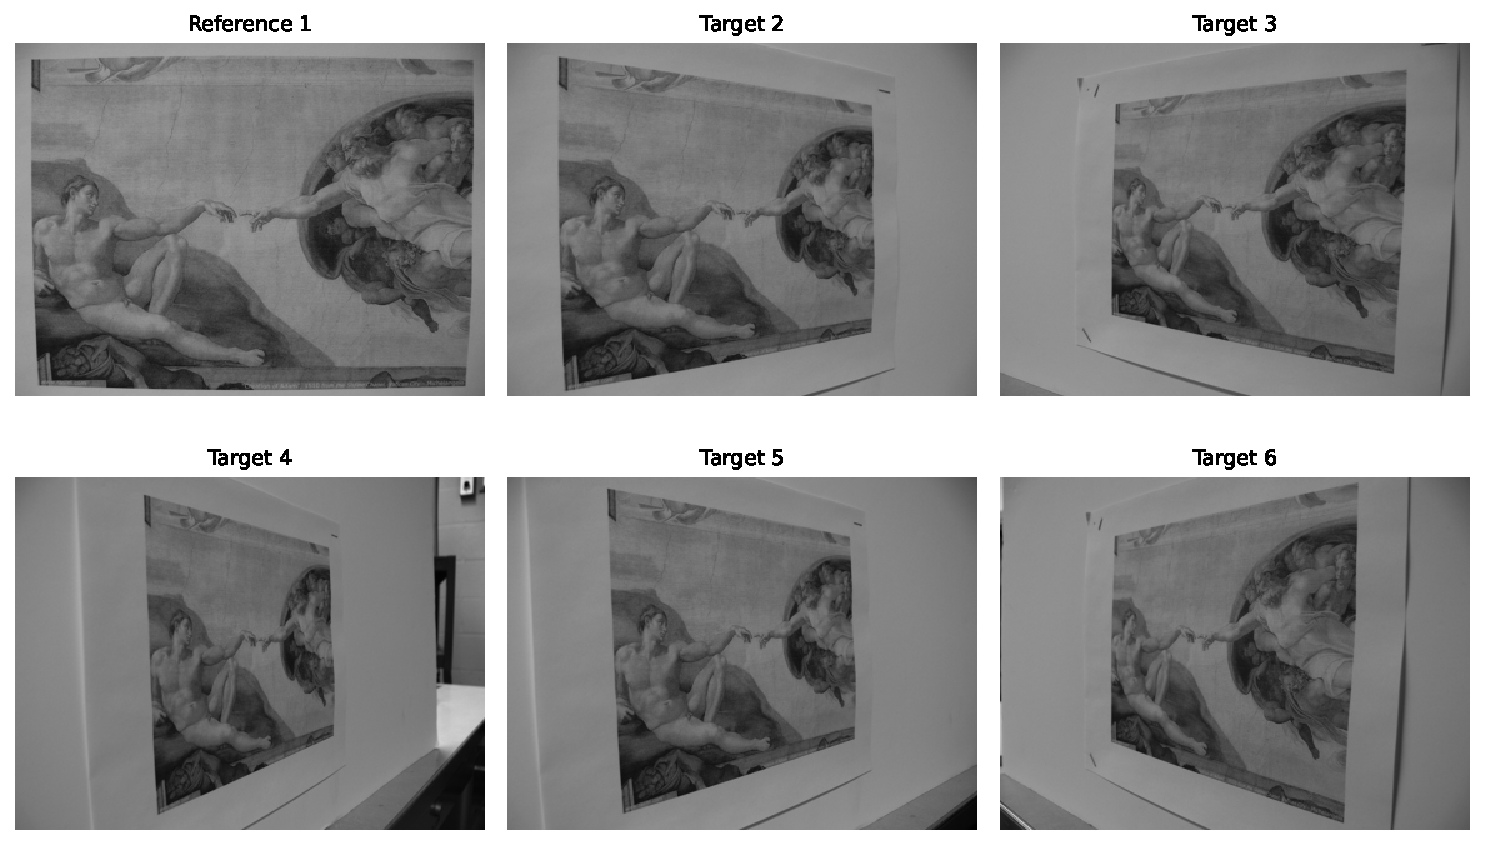
\includegraphics[width=\textwidth]{evidence/hp_13.pdf}
\caption{Actual reference and all evaluated targets for v\_adam.}\label{fig:hp-scene-13}\end{figure}

\begin{table}[H]\centering\small
\caption{Saved oracle-pair support and corner error for v\_adam.}\label{tab:hp-pairs-13}
\begin{tabular}{lrrrrrr}\toprule
Target & SIFT I & SIFT E & SIFT H5 & SP+LG I & SP+LG E & SP+LG H5 \\
\midrule
2 & 231 & 0.90 & yes & 375 & 0.53 & yes \\
3 & 173 & 0.86 & yes & 377 & 0.79 & yes \\
4 & 54 & 2.58 & yes & 259 & 1.08 & yes \\
5 & 135 & 1.66 & yes & 288 & 1.72 & yes \\
6 & 102 & 1.28 & yes & 320 & 1.07 & yes \\
\bottomrule\end{tabular}\end{table}


SIFT obtains 5 of five successful oracle homographies; SP+LG obtains 5 of five. The paired comparison contains 0 learned-only successes and 0 SIFT-only successes. Median inlier counts are 135.0 and 320.0, respectively. These support counts are computed from different tentative correspondence sets, so their magnitudes alone do not establish a more accurate mapping.

\begin{table}[H]\centering\small
\caption{Search and anchoring outcomes for the same five targets.}\label{tab:hp-end-13}
\begin{tabular}{lrrr}\toprule
Method & Rank-1 correct & Correctly verified & End-to-end H5 \\
\midrule
SIFT & 5/5 & 5/5 & 5/5 \\
SP+LG & 5/5 & 5/5 & 5/5 \\
Full & 4/5 & 4/5 & 4/5 \\
\bottomrule\end{tabular}\end{table}


The full hierarchy correctly verifies 4 of these five queries after searching the mixed 24-reference gallery. Its end-to-end column includes candidate selection and homography accuracy; the oracle table supplies the true reference directly. Any difference between those columns is therefore a search or decision effect rather than an additional illumination observation. The sequence remains one physical source of correlated targets, so five outcomes should not be treated as five independently sampled places.

\section{Sequence v\_apprentices}

This sequence belongs to the viewpoint subset and contributes five reference-to-target pairs. Its identity is reserved for the projection-head training split; learned components in the main A--D comparison retain their original pretrained weights in either case.

\begin{figure}[H]\centering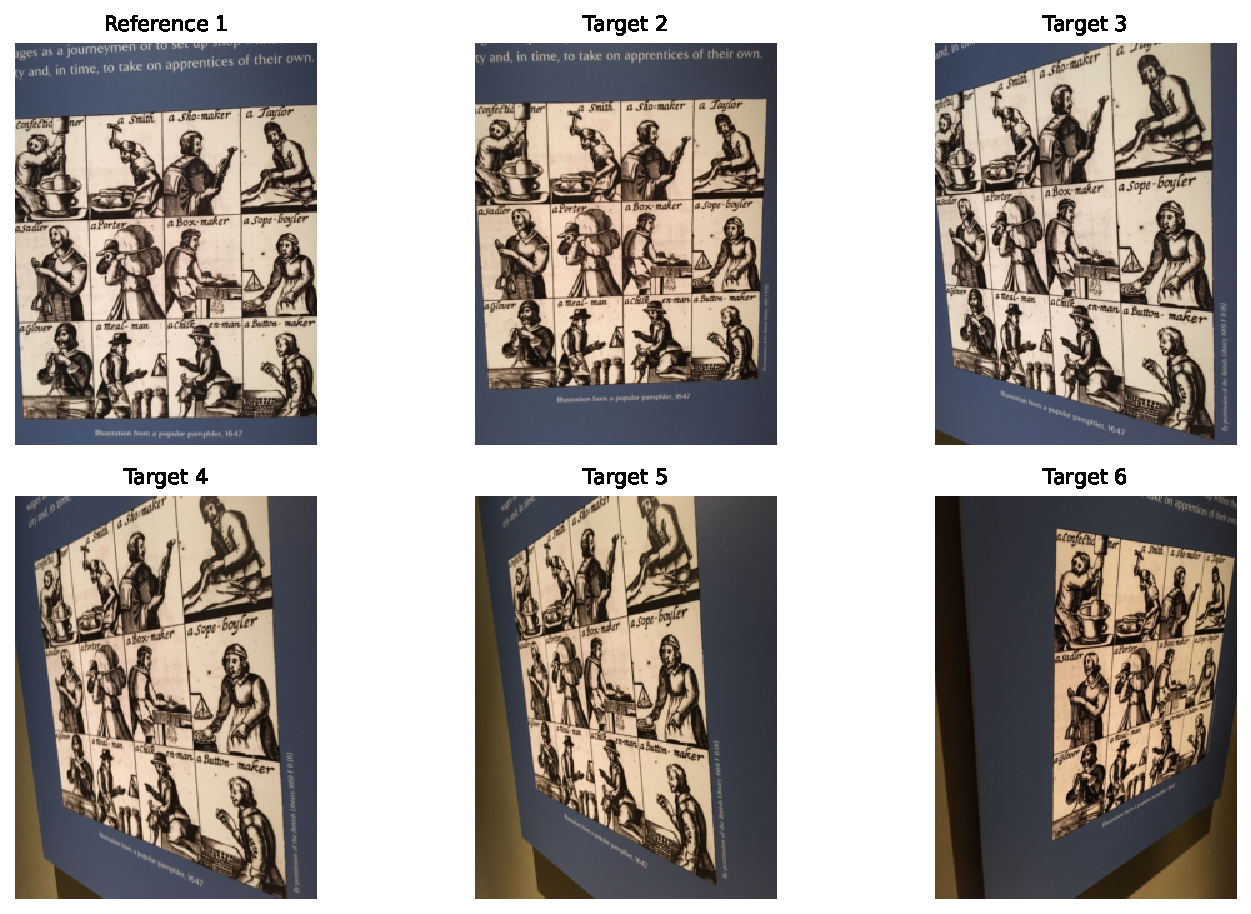
\includegraphics[width=\textwidth]{evidence/hp_14.pdf}
\caption{Actual reference and all evaluated targets for v\_apprentices.}\label{fig:hp-scene-14}\end{figure}

\begin{table}[H]\centering\small
\caption{Saved oracle-pair support and corner error for v\_apprentices.}\label{tab:hp-pairs-14}
\begin{tabular}{lrrrrrr}\toprule
Target & SIFT I & SIFT E & SIFT H5 & SP+LG I & SP+LG E & SP+LG H5 \\
\midrule
2 & 302 & 0.38 & yes & 392 & 0.22 & yes \\
3 & 223 & 0.92 & yes & 320 & 0.44 & yes \\
4 & 104 & 1.93 & yes & 282 & 0.41 & yes \\
5 & 45 & 4.00 & yes & 258 & 0.34 & yes \\
6 & 41 & 0.96 & yes & 279 & 0.47 & yes \\
\bottomrule\end{tabular}\end{table}


SIFT obtains 5 of five successful oracle homographies; SP+LG obtains 5 of five. The paired comparison contains 0 learned-only successes and 0 SIFT-only successes. Median inlier counts are 104.0 and 282.0, respectively. These support counts are computed from different tentative correspondence sets, so their magnitudes alone do not establish a more accurate mapping.

\begin{table}[H]\centering\small
\caption{Search and anchoring outcomes for the same five targets.}\label{tab:hp-end-14}
\begin{tabular}{lrrr}\toprule
Method & Rank-1 correct & Correctly verified & End-to-end H5 \\
\midrule
SIFT & 5/5 & 5/5 & 5/5 \\
SP+LG & 5/5 & 5/5 & 5/5 \\
Full & 5/5 & 5/5 & 5/5 \\
\bottomrule\end{tabular}\end{table}


The full hierarchy correctly verifies 5 of these five queries after searching the mixed 24-reference gallery. Its end-to-end column includes candidate selection and homography accuracy; the oracle table supplies the true reference directly. Any difference between those columns is therefore a search or decision effect rather than an additional illumination observation. The sequence remains one physical source of correlated targets, so five outcomes should not be treated as five independently sampled places.

\section{Sequence v\_artisans}

This sequence belongs to the viewpoint subset and contributes five reference-to-target pairs. Its identity is reserved for the projection-head training split; learned components in the main A--D comparison retain their original pretrained weights in either case.

\begin{figure}[H]\centering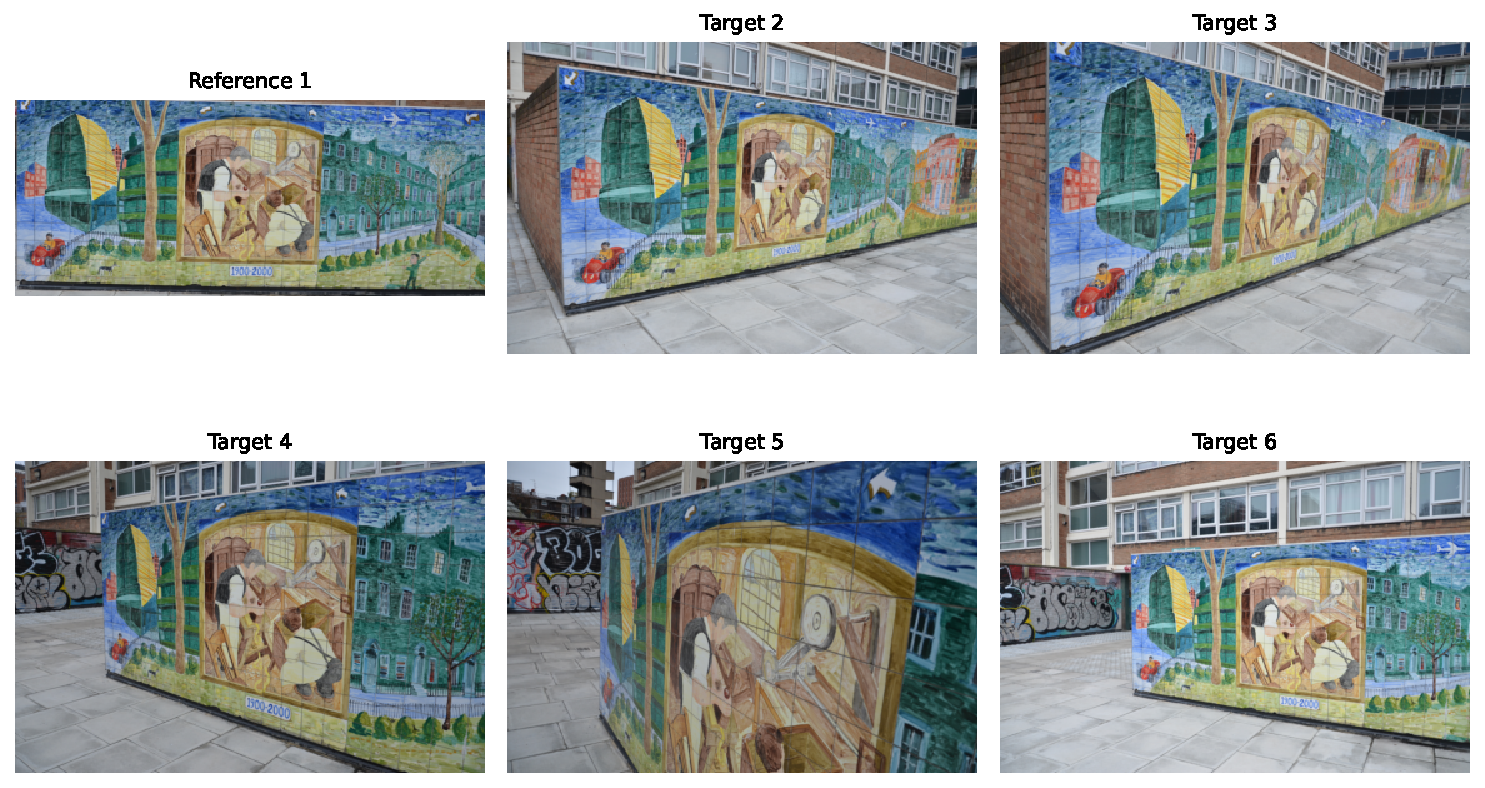
\includegraphics[width=\textwidth]{evidence/hp_15.pdf}
\caption{Actual reference and all evaluated targets for v\_artisans.}\label{fig:hp-scene-15}\end{figure}

\begin{table}[H]\centering\small
\caption{Saved oracle-pair support and corner error for v\_artisans.}\label{tab:hp-pairs-15}
\begin{tabular}{lrrrrrr}\toprule
Target & SIFT I & SIFT E & SIFT H5 & SP+LG I & SP+LG E & SP+LG H5 \\
\midrule
2 & 125 & 0.42 & yes & 243 & 0.35 & yes \\
3 & 87 & 1.20 & yes & 209 & 0.93 & yes \\
4 & 84 & 4.22 & yes & 248 & 1.54 & yes \\
5 & 8 & -- & no & 109 & -- & no \\
6 & 116 & 0.40 & yes & 260 & 0.36 & yes \\
\bottomrule\end{tabular}\end{table}


SIFT obtains 4 of five successful oracle homographies; SP+LG obtains 4 of five. The paired comparison contains 0 learned-only successes and 0 SIFT-only successes. Median inlier counts are 87.0 and 243.0, respectively. These support counts are computed from different tentative correspondence sets, so their magnitudes alone do not establish a more accurate mapping.

\begin{table}[H]\centering\small
\caption{Search and anchoring outcomes for the same five targets.}\label{tab:hp-end-15}
\begin{tabular}{lrrr}\toprule
Method & Rank-1 correct & Correctly verified & End-to-end H5 \\
\midrule
SIFT & 5/5 & 4/5 & 4/5 \\
SP+LG & 5/5 & 4/5 & 4/5 \\
Full & 4/5 & 3/5 & 3/5 \\
\bottomrule\end{tabular}\end{table}


The full hierarchy correctly verifies 3 of these five queries after searching the mixed 24-reference gallery. Its end-to-end column includes candidate selection and homography accuracy; the oracle table supplies the true reference directly. Any difference between those columns is therefore a search or decision effect rather than an additional illumination observation. The sequence remains one physical source of correlated targets, so five outcomes should not be treated as five independently sampled places.

\section{Sequence v\_astronautis}

This sequence belongs to the viewpoint subset and contributes five reference-to-target pairs. Its identity is held out from projection-head training; learned components in the main A--D comparison retain their original pretrained weights in either case.

\begin{figure}[H]\centering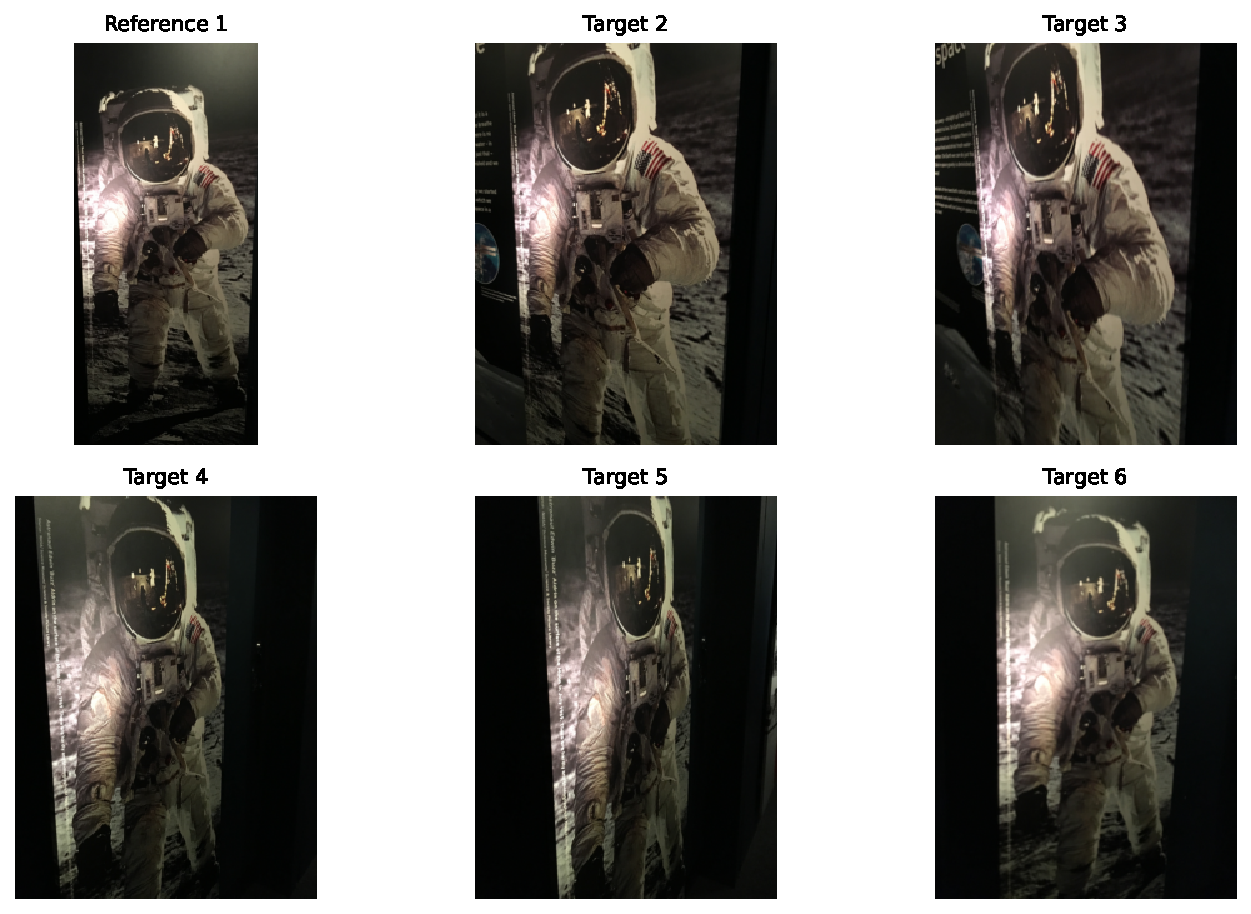
\includegraphics[width=\textwidth]{evidence/hp_16.pdf}
\caption{Actual reference and all evaluated targets for v\_astronautis.}\label{fig:hp-scene-16}\end{figure}

\begin{table}[H]\centering\small
\caption{Saved oracle-pair support and corner error for v\_astronautis.}\label{tab:hp-pairs-16}
\begin{tabular}{lrrrrrr}\toprule
Target & SIFT I & SIFT E & SIFT H5 & SP+LG I & SP+LG E & SP+LG H5 \\
\midrule
2 & 162 & 1.35 & yes & 307 & 1.02 & yes \\
3 & 51 & 5.82 & no & 236 & 1.08 & yes \\
4 & 83 & 1.10 & yes & 305 & 0.72 & yes \\
5 & 21 & 2.80 & yes & 203 & 7.21 & no \\
6 & 160 & 1.12 & yes & 298 & 3.44 & yes \\
\bottomrule\end{tabular}\end{table}


SIFT obtains 4 of five successful oracle homographies; SP+LG obtains 4 of five. The paired comparison contains 1 learned-only success and 1 SIFT-only success. Median inlier counts are 83.0 and 298.0, respectively. These support counts are computed from different tentative correspondence sets, so their magnitudes alone do not establish a more accurate mapping.

\begin{table}[H]\centering\small
\caption{Search and anchoring outcomes for the same five targets.}\label{tab:hp-end-16}
\begin{tabular}{lrrr}\toprule
Method & Rank-1 correct & Correctly verified & End-to-end H5 \\
\midrule
SIFT & 5/5 & 5/5 & 4/5 \\
SP+LG & 5/5 & 5/5 & 4/5 \\
Full & 3/5 & 3/5 & 3/5 \\
\bottomrule\end{tabular}\end{table}


The full hierarchy correctly verifies 3 of these five queries after searching the mixed 24-reference gallery. Its end-to-end column includes candidate selection and homography accuracy; the oracle table supplies the true reference directly. Any difference between those columns is therefore a search or decision effect rather than an additional illumination observation. The sequence remains one physical source of correlated targets, so five outcomes should not be treated as five independently sampled places.

\section{Sequence v\_azzola}

This sequence belongs to the viewpoint subset and contributes five reference-to-target pairs. Its identity is held out from projection-head training; learned components in the main A--D comparison retain their original pretrained weights in either case.

\begin{figure}[H]\centering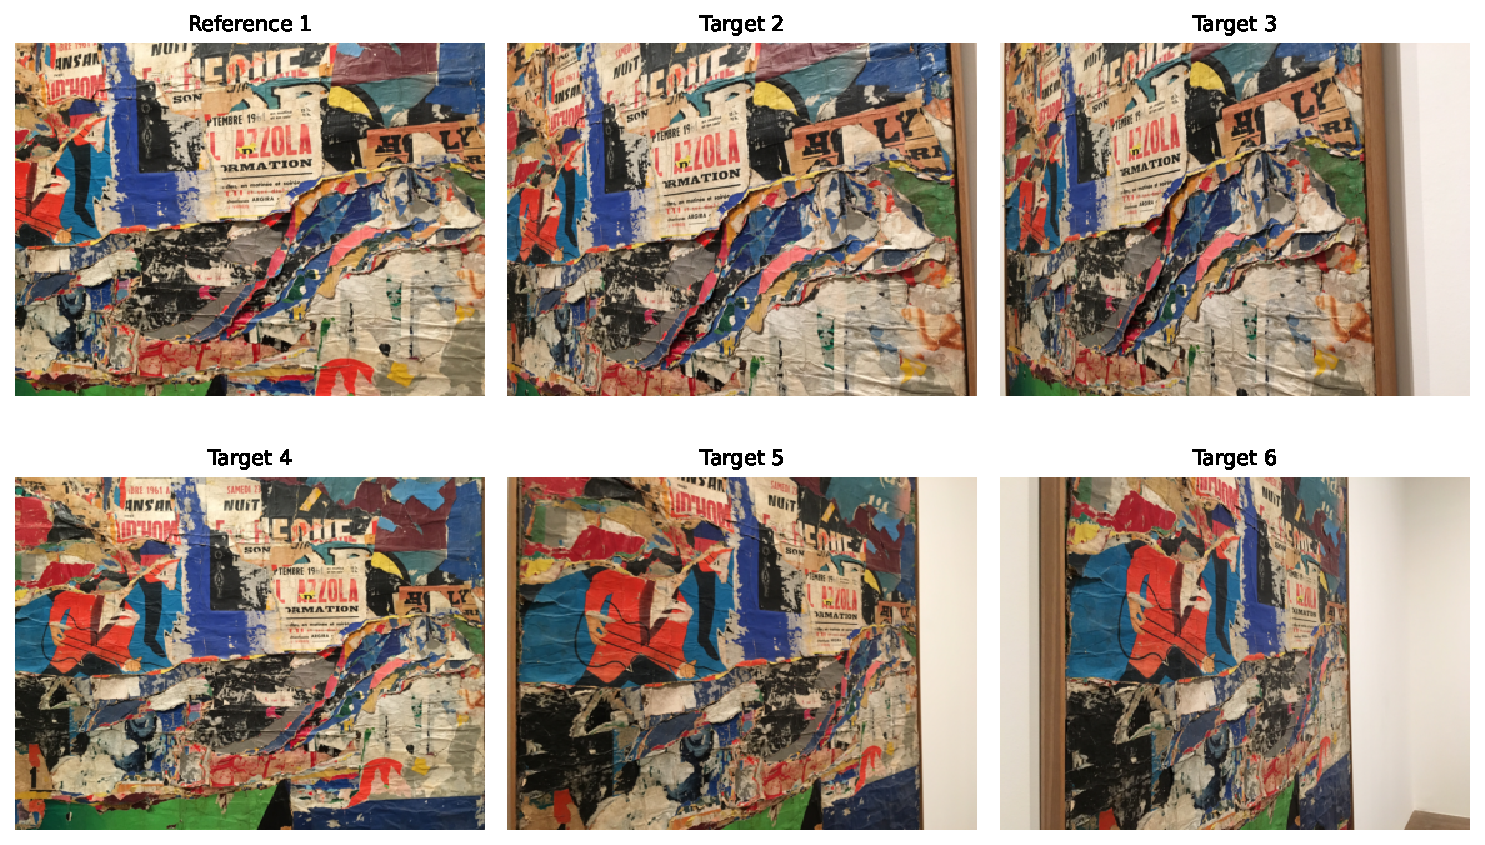
\includegraphics[width=\textwidth]{evidence/hp_17.pdf}
\caption{Actual reference and all evaluated targets for v\_azzola.}\label{fig:hp-scene-17}\end{figure}

\begin{table}[H]\centering\small
\caption{Saved oracle-pair support and corner error for v\_azzola.}\label{tab:hp-pairs-17}
\begin{tabular}{lrrrrrr}\toprule
Target & SIFT I & SIFT E & SIFT H5 & SP+LG I & SP+LG E & SP+LG H5 \\
\midrule
2 & 164 & 1.99 & yes & 217 & 1.58 & yes \\
3 & 33 & 3.56 & yes & 199 & 2.63 & yes \\
4 & 278 & 0.91 & yes & 249 & 0.64 & yes \\
5 & 60 & 5.79 & no & 168 & 1.83 & yes \\
6 & 6 & 20.65 & no & 107 & 3.76 & yes \\
\bottomrule\end{tabular}\end{table}


SIFT obtains 3 of five successful oracle homographies; SP+LG obtains 5 of five. The paired comparison contains 2 learned-only successes and 0 SIFT-only successes. Median inlier counts are 60.0 and 199.0, respectively. These support counts are computed from different tentative correspondence sets, so their magnitudes alone do not establish a more accurate mapping.

\begin{table}[H]\centering\small
\caption{Search and anchoring outcomes for the same five targets.}\label{tab:hp-end-17}
\begin{tabular}{lrrr}\toprule
Method & Rank-1 correct & Correctly verified & End-to-end H5 \\
\midrule
SIFT & 4/5 & 4/5 & 3/5 \\
SP+LG & 5/5 & 5/5 & 5/5 \\
Full & 4/5 & 4/5 & 4/5 \\
\bottomrule\end{tabular}\end{table}


The full hierarchy correctly verifies 4 of these five queries after searching the mixed 24-reference gallery. Its end-to-end column includes candidate selection and homography accuracy; the oracle table supplies the true reference directly. Any difference between those columns is therefore a search or decision effect rather than an additional illumination observation. The sequence remains one physical source of correlated targets, so five outcomes should not be treated as five independently sampled places.

\section{Sequence v\_bark}

This sequence belongs to the viewpoint subset and contributes five reference-to-target pairs. Its identity is held out from projection-head training; learned components in the main A--D comparison retain their original pretrained weights in either case.

\begin{figure}[H]\centering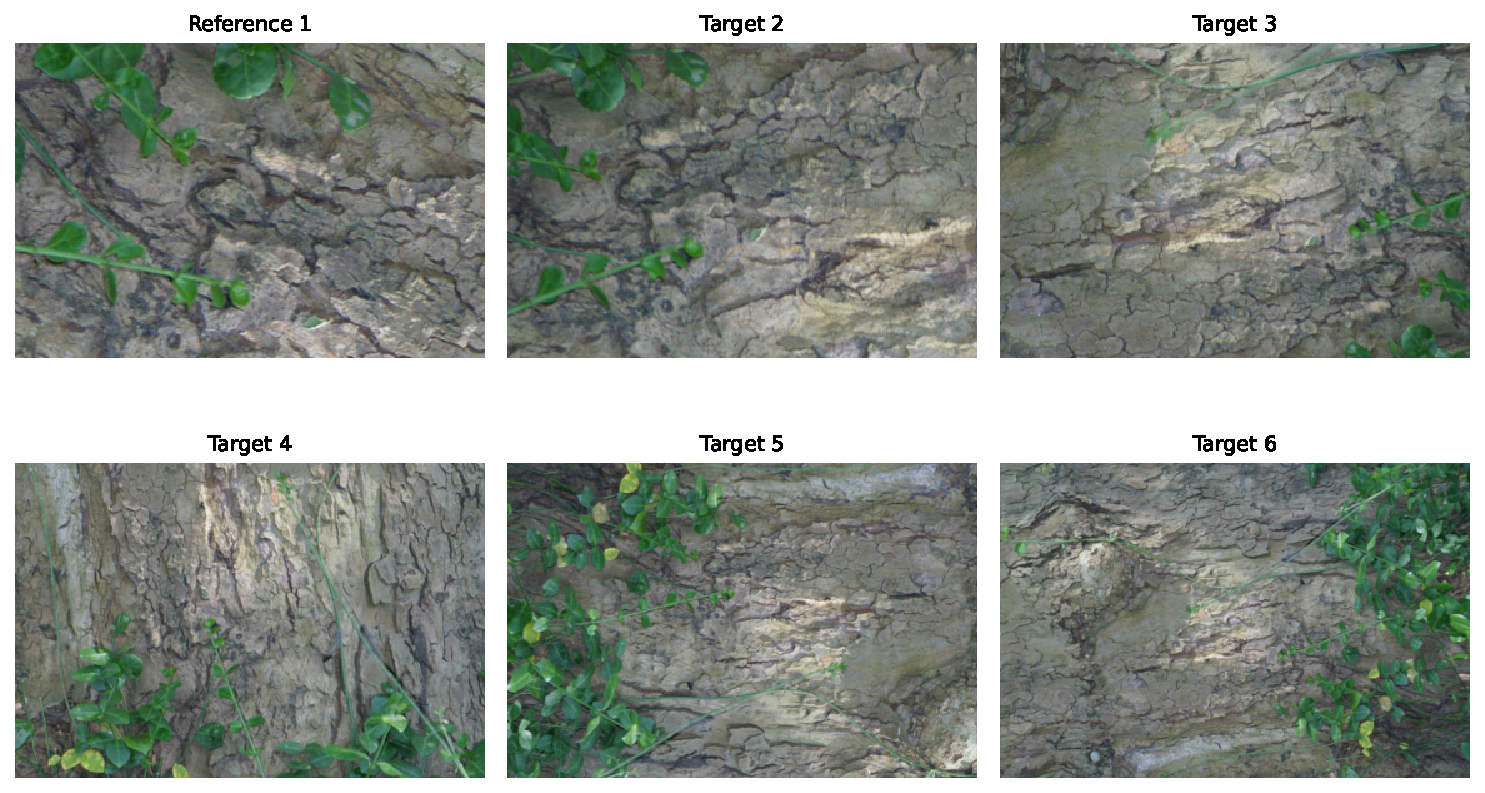
\includegraphics[width=\textwidth]{evidence/hp_18.pdf}
\caption{Actual reference and all evaluated targets for v\_bark.}\label{fig:hp-scene-18}\end{figure}

\begin{table}[H]\centering\small
\caption{Saved oracle-pair support and corner error for v\_bark.}\label{tab:hp-pairs-18}
\begin{tabular}{lrrrrrr}\toprule
Target & SIFT I & SIFT E & SIFT H5 & SP+LG I & SP+LG E & SP+LG H5 \\
\midrule
2 & 116 & 0.41 & yes & 240 & 0.66 & yes \\
3 & 73 & 0.67 & yes & 4 & -- & no \\
4 & 53 & 0.41 & yes & 5 & 451.46 & no \\
5 & 47 & 0.54 & yes & 41 & 1.38 & yes \\
6 & 23 & 0.46 & yes & 5 & 495.20 & no \\
\bottomrule\end{tabular}\end{table}


SIFT obtains 5 of five successful oracle homographies; SP+LG obtains 2 of five. The paired comparison contains 0 learned-only successes and 3 SIFT-only successes. Median inlier counts are 53.0 and 5.0, respectively. These support counts are computed from different tentative correspondence sets, so their magnitudes alone do not establish a more accurate mapping.

\begin{table}[H]\centering\small
\caption{Search and anchoring outcomes for the same five targets.}\label{tab:hp-end-18}
\begin{tabular}{lrrr}\toprule
Method & Rank-1 correct & Correctly verified & End-to-end H5 \\
\midrule
SIFT & 5/5 & 5/5 & 5/5 \\
SP+LG & 2/5 & 2/5 & 2/5 \\
Full & 3/5 & 2/5 & 2/5 \\
\bottomrule\end{tabular}\end{table}


The full hierarchy correctly verifies 2 of these five queries after searching the mixed 24-reference gallery. Its end-to-end column includes candidate selection and homography accuracy; the oracle table supplies the true reference directly. Any difference between those columns is therefore a search or decision effect rather than an additional illumination observation. The sequence remains one physical source of correlated targets, so five outcomes should not be treated as five independently sampled places.

\section{Sequence v\_bees}

This sequence belongs to the viewpoint subset and contributes five reference-to-target pairs. Its identity is held out from projection-head training; learned components in the main A--D comparison retain their original pretrained weights in either case.

\begin{figure}[H]\centering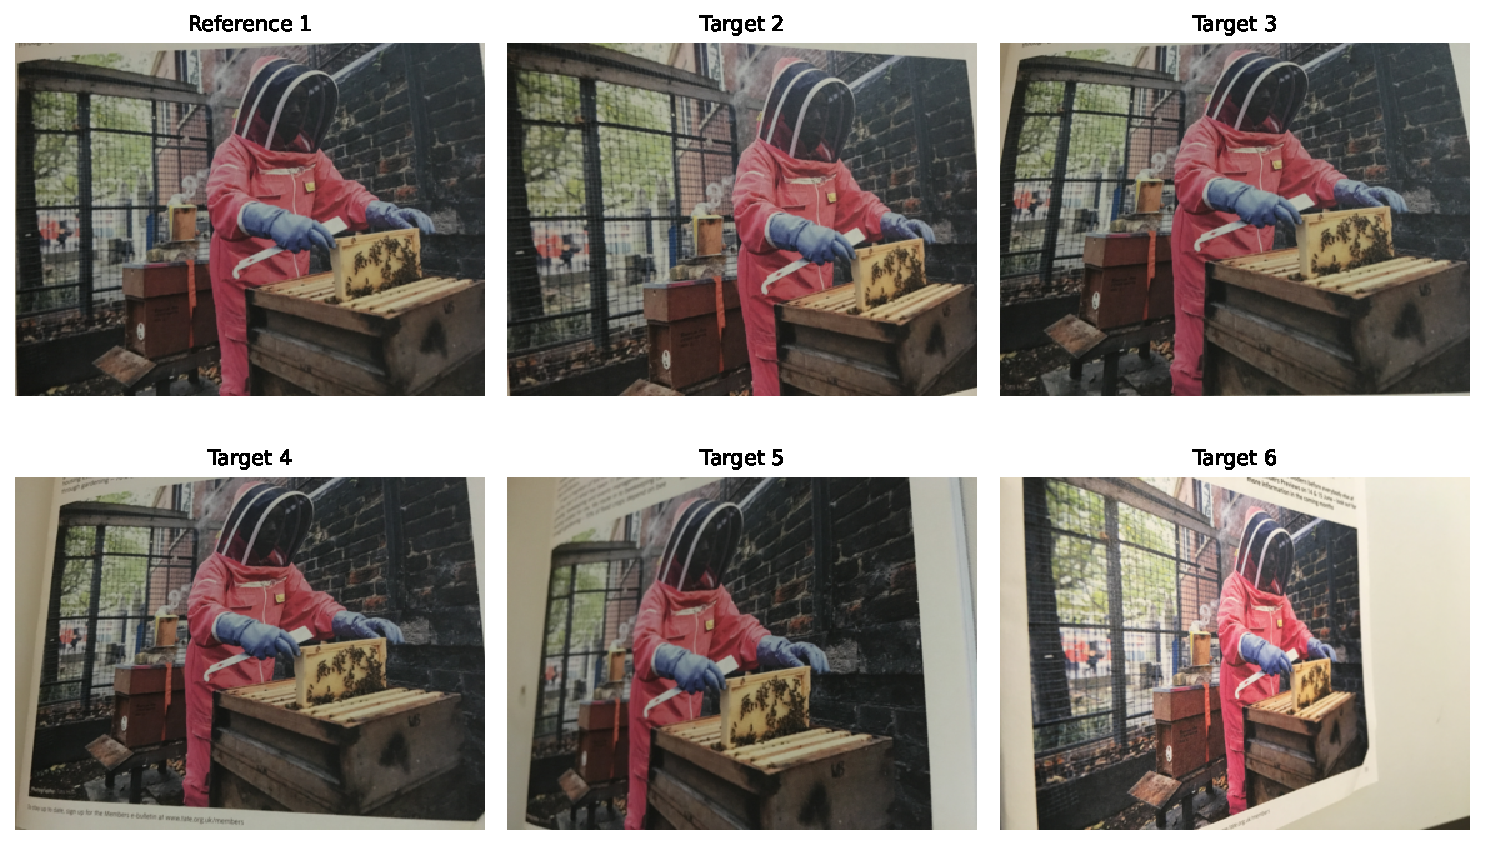
\includegraphics[width=\textwidth]{evidence/hp_19.pdf}
\caption{Actual reference and all evaluated targets for v\_bees.}\label{fig:hp-scene-19}\end{figure}

\begin{table}[H]\centering\small
\caption{Saved oracle-pair support and corner error for v\_bees.}\label{tab:hp-pairs-19}
\begin{tabular}{lrrrrrr}\toprule
Target & SIFT I & SIFT E & SIFT H5 & SP+LG I & SP+LG E & SP+LG H5 \\
\midrule
2 & 307 & 0.43 & yes & 368 & 0.70 & yes \\
3 & 341 & 0.23 & yes & 401 & 0.47 & yes \\
4 & 304 & 0.44 & yes & 342 & 0.90 & yes \\
5 & 161 & 0.84 & yes & 231 & 2.14 & yes \\
6 & 166 & 1.86 & yes & 325 & 0.96 & yes \\
\bottomrule\end{tabular}\end{table}


SIFT obtains 5 of five successful oracle homographies; SP+LG obtains 5 of five. The paired comparison contains 0 learned-only successes and 0 SIFT-only successes. Median inlier counts are 304.0 and 342.0, respectively. These support counts are computed from different tentative correspondence sets, so their magnitudes alone do not establish a more accurate mapping.

\begin{table}[H]\centering\small
\caption{Search and anchoring outcomes for the same five targets.}\label{tab:hp-end-19}
\begin{tabular}{lrrr}\toprule
Method & Rank-1 correct & Correctly verified & End-to-end H5 \\
\midrule
SIFT & 5/5 & 5/5 & 5/5 \\
SP+LG & 5/5 & 5/5 & 5/5 \\
Full & 5/5 & 5/5 & 5/5 \\
\bottomrule\end{tabular}\end{table}


The full hierarchy correctly verifies 5 of these five queries after searching the mixed 24-reference gallery. Its end-to-end column includes candidate selection and homography accuracy; the oracle table supplies the true reference directly. Any difference between those columns is therefore a search or decision effect rather than an additional illumination observation. The sequence remains one physical source of correlated targets, so five outcomes should not be treated as five independently sampled places.

\section{Sequence v\_beyus}

This sequence belongs to the viewpoint subset and contributes five reference-to-target pairs. Its identity is held out from projection-head training; learned components in the main A--D comparison retain their original pretrained weights in either case.

\begin{figure}[H]\centering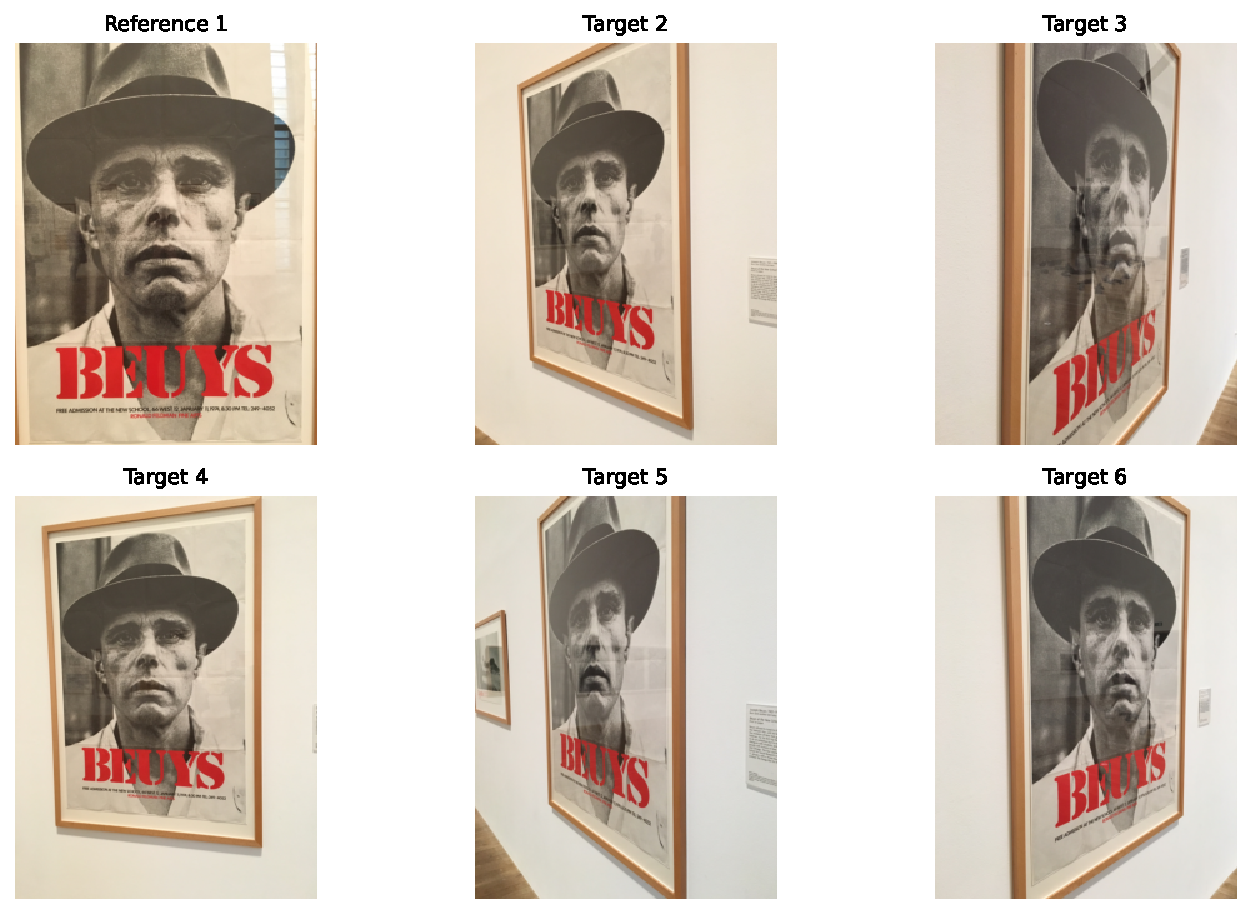
\includegraphics[width=\textwidth]{evidence/hp_20.pdf}
\caption{Actual reference and all evaluated targets for v\_beyus.}\label{fig:hp-scene-20}\end{figure}

\begin{table}[H]\centering\small
\caption{Saved oracle-pair support and corner error for v\_beyus.}\label{tab:hp-pairs-20}
\begin{tabular}{lrrrrrr}\toprule
Target & SIFT I & SIFT E & SIFT H5 & SP+LG I & SP+LG E & SP+LG H5 \\
\midrule
2 & 93 & 0.58 & yes & 217 & 0.98 & yes \\
3 & 9 & 43.75 & no & 189 & 1.51 & yes \\
4 & 230 & 0.23 & yes & 281 & 0.32 & yes \\
5 & 14 & 5.91 & no & 158 & 2.00 & yes \\
6 & 37 & 1.80 & yes & 211 & 1.34 & yes \\
\bottomrule\end{tabular}\end{table}


SIFT obtains 3 of five successful oracle homographies; SP+LG obtains 5 of five. The paired comparison contains 2 learned-only successes and 0 SIFT-only successes. Median inlier counts are 37.0 and 211.0, respectively. These support counts are computed from different tentative correspondence sets, so their magnitudes alone do not establish a more accurate mapping.

\begin{table}[H]\centering\small
\caption{Search and anchoring outcomes for the same five targets.}\label{tab:hp-end-20}
\begin{tabular}{lrrr}\toprule
Method & Rank-1 correct & Correctly verified & End-to-end H5 \\
\midrule
SIFT & 5/5 & 4/5 & 3/5 \\
SP+LG & 5/5 & 5/5 & 5/5 \\
Full & 5/5 & 5/5 & 5/5 \\
\bottomrule\end{tabular}\end{table}


The full hierarchy correctly verifies 5 of these five queries after searching the mixed 24-reference gallery. Its end-to-end column includes candidate selection and homography accuracy; the oracle table supplies the true reference directly. Any difference between those columns is therefore a search or decision effect rather than an additional illumination observation. The sequence remains one physical source of correlated targets, so five outcomes should not be treated as five independently sampled places.

\section{Sequence v\_bip}

This sequence belongs to the viewpoint subset and contributes five reference-to-target pairs. Its identity is held out from projection-head training; learned components in the main A--D comparison retain their original pretrained weights in either case.

\begin{figure}[H]\centering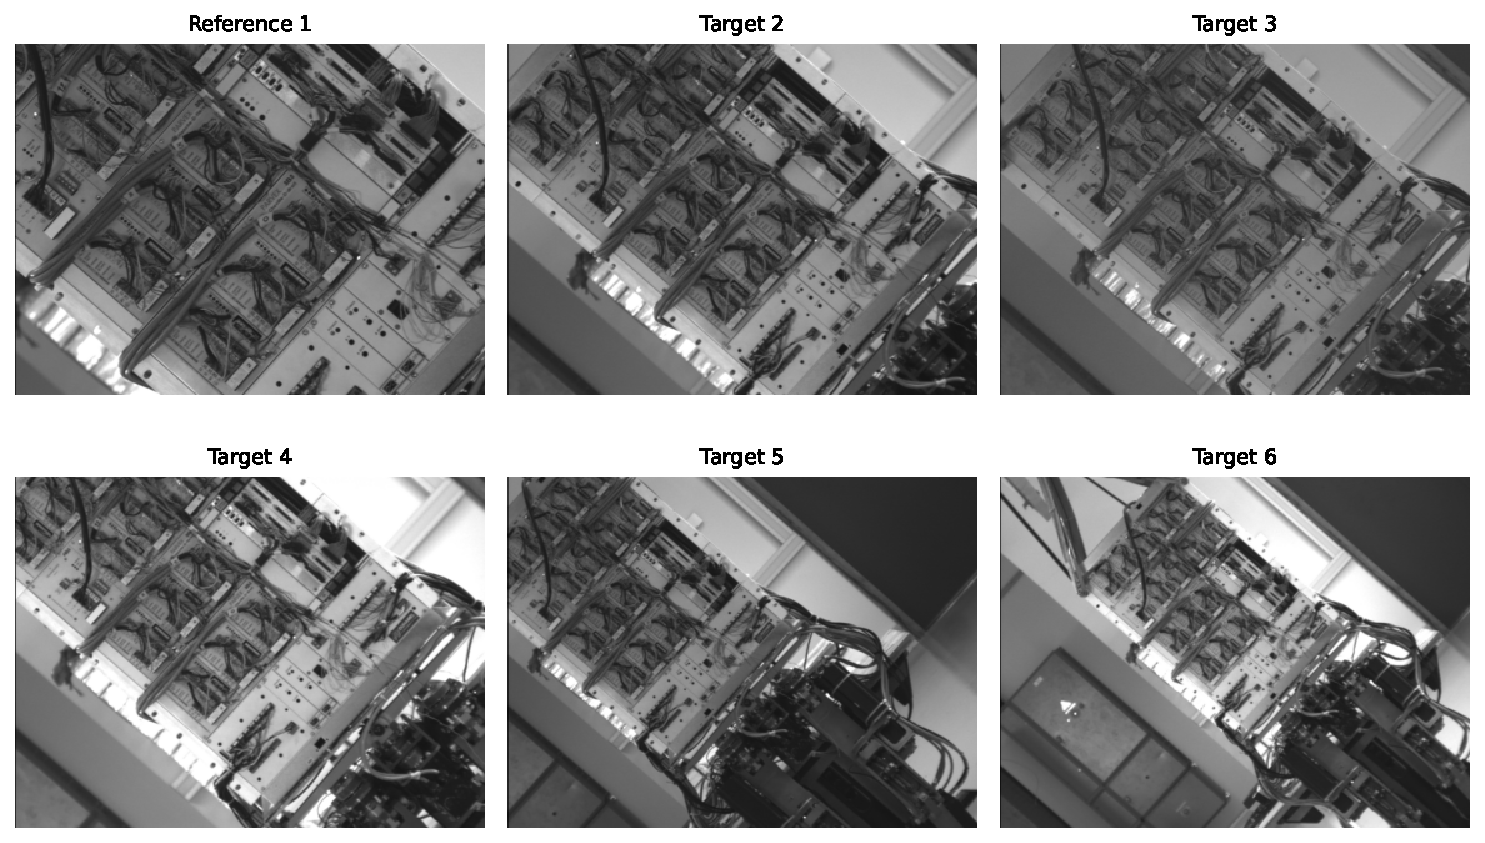
\includegraphics[width=\textwidth]{evidence/hp_21.pdf}
\caption{Actual reference and all evaluated targets for v\_bip.}\label{fig:hp-scene-21}\end{figure}

\begin{table}[H]\centering\small
\caption{Saved oracle-pair support and corner error for v\_bip.}\label{tab:hp-pairs-21}
\begin{tabular}{lrrrrrr}\toprule
Target & SIFT I & SIFT E & SIFT H5 & SP+LG I & SP+LG E & SP+LG H5 \\
\midrule
2 & 173 & 0.32 & yes & 227 & 0.38 & yes \\
3 & 140 & 0.20 & yes & 180 & 0.68 & yes \\
4 & 146 & 0.38 & yes & 187 & 0.36 & yes \\
5 & 88 & 1.86 & yes & 7 & 5.71 & no \\
6 & 78 & 0.56 & yes & 4 & -- & no \\
\bottomrule\end{tabular}\end{table}


SIFT obtains 5 of five successful oracle homographies; SP+LG obtains 3 of five. The paired comparison contains 0 learned-only successes and 2 SIFT-only successes. Median inlier counts are 140.0 and 180.0, respectively. These support counts are computed from different tentative correspondence sets, so their magnitudes alone do not establish a more accurate mapping.

\begin{table}[H]\centering\small
\caption{Search and anchoring outcomes for the same five targets.}\label{tab:hp-end-21}
\begin{tabular}{lrrr}\toprule
Method & Rank-1 correct & Correctly verified & End-to-end H5 \\
\midrule
SIFT & 5/5 & 5/5 & 5/5 \\
SP+LG & 3/5 & 3/5 & 3/5 \\
Full & 4/5 & 3/5 & 3/5 \\
\bottomrule\end{tabular}\end{table}


The full hierarchy correctly verifies 3 of these five queries after searching the mixed 24-reference gallery. Its end-to-end column includes candidate selection and homography accuracy; the oracle table supplies the true reference directly. Any difference between those columns is therefore a search or decision effect rather than an additional illumination observation. The sequence remains one physical source of correlated targets, so five outcomes should not be treated as five independently sampled places.

\section{Sequence v\_bird}

This sequence belongs to the viewpoint subset and contributes five reference-to-target pairs. Its identity is held out from projection-head training; learned components in the main A--D comparison retain their original pretrained weights in either case.

\begin{figure}[H]\centering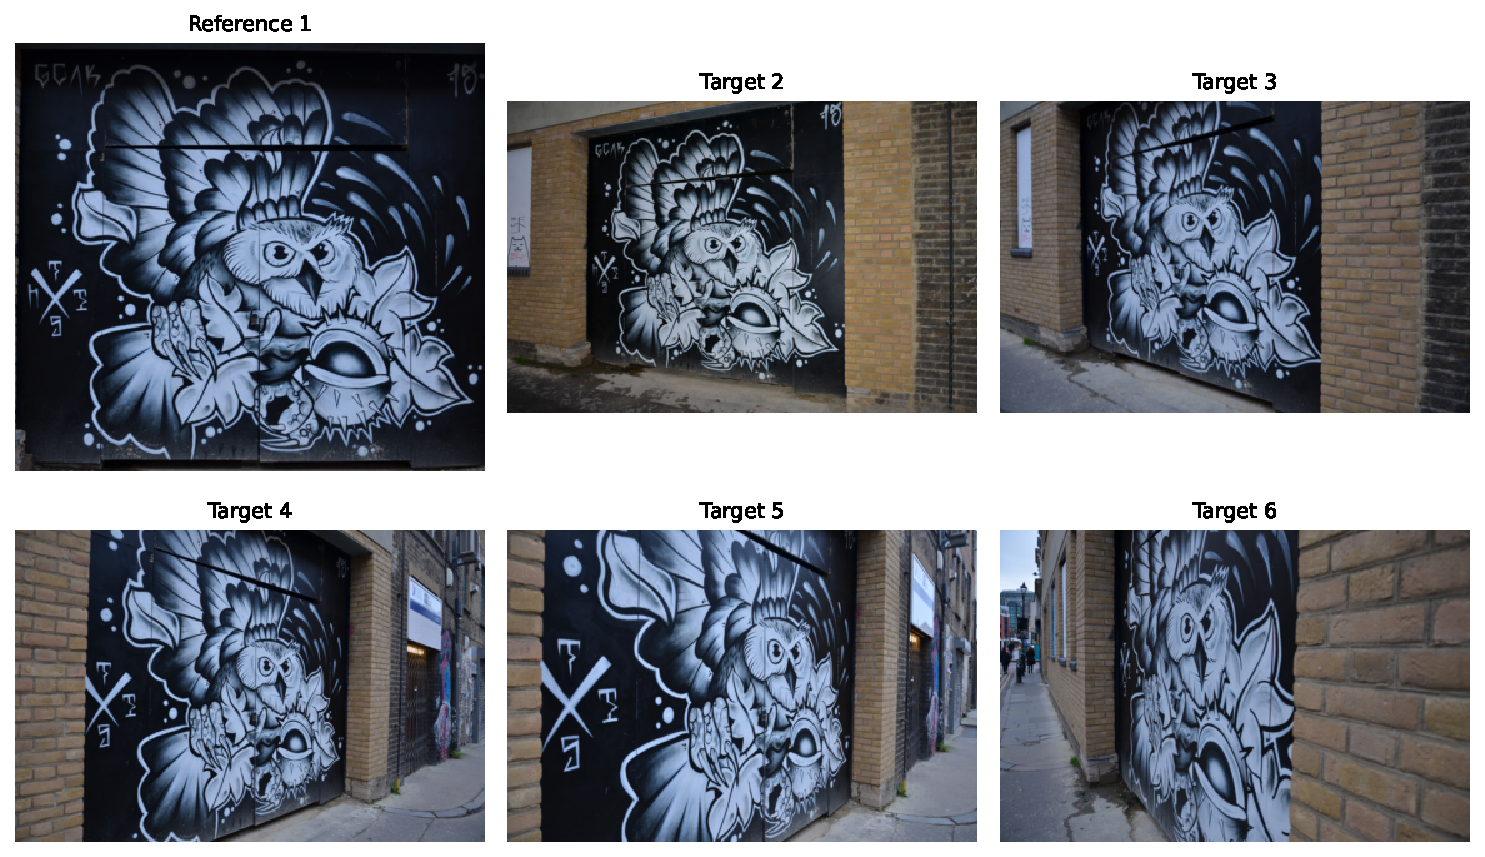
\includegraphics[width=\textwidth]{evidence/hp_22.pdf}
\caption{Actual reference and all evaluated targets for v\_bird.}\label{fig:hp-scene-22}\end{figure}

\begin{table}[H]\centering\small
\caption{Saved oracle-pair support and corner error for v\_bird.}\label{tab:hp-pairs-22}
\begin{tabular}{lrrrrrr}\toprule
Target & SIFT I & SIFT E & SIFT H5 & SP+LG I & SP+LG E & SP+LG H5 \\
\midrule
2 & 206 & 0.38 & yes & 190 & 0.36 & yes \\
3 & 129 & 1.20 & yes & 173 & 1.99 & yes \\
4 & 120 & 2.20 & yes & 214 & 1.65 & yes \\
5 & 53 & 14.30 & no & 172 & 4.15 & yes \\
6 & 4 & -- & no & 126 & 26.82 & no \\
\bottomrule\end{tabular}\end{table}


SIFT obtains 3 of five successful oracle homographies; SP+LG obtains 4 of five. The paired comparison contains 1 learned-only success and 0 SIFT-only successes. Median inlier counts are 120.0 and 173.0, respectively. These support counts are computed from different tentative correspondence sets, so their magnitudes alone do not establish a more accurate mapping.

\begin{table}[H]\centering\small
\caption{Search and anchoring outcomes for the same five targets.}\label{tab:hp-end-22}
\begin{tabular}{lrrr}\toprule
Method & Rank-1 correct & Correctly verified & End-to-end H5 \\
\midrule
SIFT & 4/5 & 4/5 & 3/5 \\
SP+LG & 5/5 & 5/5 & 4/5 \\
Full & 3/5 & 3/5 & 3/5 \\
\bottomrule\end{tabular}\end{table}


The full hierarchy correctly verifies 3 of these five queries after searching the mixed 24-reference gallery. Its end-to-end column includes candidate selection and homography accuracy; the oracle table supplies the true reference directly. Any difference between those columns is therefore a search or decision effect rather than an additional illumination observation. The sequence remains one physical source of correlated targets, so five outcomes should not be treated as five independently sampled places.

\section{Sequence v\_birdwoman}

This sequence belongs to the viewpoint subset and contributes five reference-to-target pairs. Its identity is held out from projection-head training; learned components in the main A--D comparison retain their original pretrained weights in either case.

\begin{figure}[H]\centering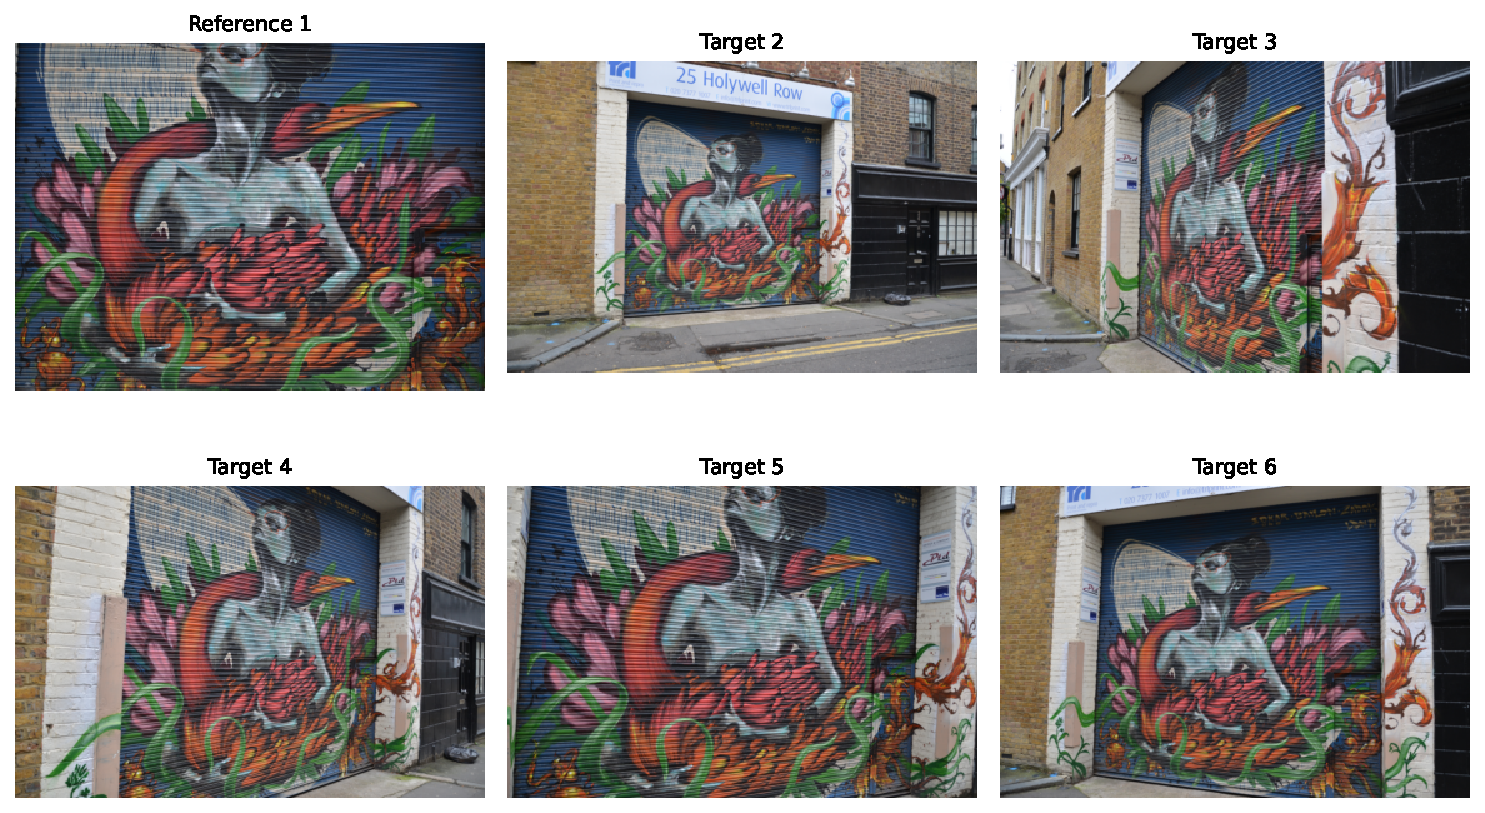
\includegraphics[width=\textwidth]{evidence/hp_23.pdf}
\caption{Actual reference and all evaluated targets for v\_birdwoman.}\label{fig:hp-scene-23}\end{figure}

\begin{table}[H]\centering\small
\caption{Saved oracle-pair support and corner error for v\_birdwoman.}\label{tab:hp-pairs-23}
\begin{tabular}{lrrrrrr}\toprule
Target & SIFT I & SIFT E & SIFT H5 & SP+LG I & SP+LG E & SP+LG H5 \\
\midrule
2 & 22 & 0.94 & yes & 49 & 1.47 & yes \\
3 & 26 & 4.65 & yes & 82 & 2.11 & yes \\
4 & 84 & 0.79 & yes & 91 & 0.91 & yes \\
5 & 240 & 0.29 & yes & 219 & 0.28 & yes \\
6 & 50 & 0.80 & yes & 106 & 0.98 & yes \\
\bottomrule\end{tabular}\end{table}


SIFT obtains 5 of five successful oracle homographies; SP+LG obtains 5 of five. The paired comparison contains 0 learned-only successes and 0 SIFT-only successes. Median inlier counts are 50.0 and 91.0, respectively. These support counts are computed from different tentative correspondence sets, so their magnitudes alone do not establish a more accurate mapping.

\begin{table}[H]\centering\small
\caption{Search and anchoring outcomes for the same five targets.}\label{tab:hp-end-23}
\begin{tabular}{lrrr}\toprule
Method & Rank-1 correct & Correctly verified & End-to-end H5 \\
\midrule
SIFT & 5/5 & 5/5 & 5/5 \\
SP+LG & 5/5 & 5/5 & 5/5 \\
Full & 5/5 & 5/5 & 5/5 \\
\bottomrule\end{tabular}\end{table}


The full hierarchy correctly verifies 5 of these five queries after searching the mixed 24-reference gallery. Its end-to-end column includes candidate selection and homography accuracy; the oracle table supplies the true reference directly. Any difference between those columns is therefore a search or decision effect rather than an additional illumination observation. The sequence remains one physical source of correlated targets, so five outcomes should not be treated as five independently sampled places.
